% Template for PLoS
% Version 1.0 January 2009
%
% To compile to pdf, run:
% latex plos.template
% bibtex plos.template
% latex plos.template
% latex plos.template
% dvipdf plos.template

\documentclass[10pt]{article}

% amsmath package, useful for mathematical formulas
\usepackage{amsmath}
% amssymb package, useful for mathematical symbols
\usepackage{amssymb}

\usepackage{soul}

% graphicx package, useful for including eps and pdf graphics
% include graphics with the command \includegraphics
\usepackage{graphicx}

% cite package, to clean up citations in the main text. Do not remove.
\usepackage{cite}

\usepackage{color} 

\usepackage{hyperref} 

% Use doublespacing - comment out for single spacing
\usepackage{setspace} 
\doublespacing


% Text layout
\topmargin 0.0cm
\oddsidemargin 0.5cm
\evensidemargin 0.5cm
\textwidth 16cm 
\textheight 21cm

% Bold the 'Figure #' in the caption and separate it with a period
% Captions will be left justified
\usepackage[labelfont=bf,labelsep=period,justification=raggedright]{caption}

% Use the PLoS provided bibtex style
%\bibliographystyle{abbrv}
\bibliographystyle{plos2015}

% Remove brackets from numbering in List of References
\makeatletter
\renewcommand{\@biblabel}[1]{\quad#1.}
\makeatother


% Leave date blank
\date{}

\pagestyle{myheadings}
%% ** EDIT HERE **

% bold in tables
\usepackage{array}
% \newcolumntype{$}{>{\global\let\currentrowstyle\relax}} ## commented to avoid errors when counting words
\newcolumntype{^}{>{\currentrowstyle}}
\newcommand{\rowstyle}[1]{\gdef\currentrowstyle{#1}%
  #1\ignorespaces
}

%% ** EDIT HERE **
%% PLEASE INCLUDE ALL MACROS BELOW

%% END MACROS SECTION

\begin{document}

%% Title must be 150 characters or less
\begin{flushleft}
{\Large
\textbf{Summary Statistics Based Method to Infer Phenotypic Consequences of Gene Regulation}
}
% Insert Author names, affiliations and corresponding author email.

Alvaro Barbeira$^{1}$,
Scott P. Dickinson$^{1}$,
Jason M. Torres$^{2}$,
Eric S. Torstenson$^{3}$,
Jiamao Zheng $^{1}$,
Heather E. Wheeler$^4$,
Kaanan P. Shah$^{1}$, 
Todd Edwards$^{3}$,
%%##Tzintzuni Garcia$^{5}$,
%GTEx Consortium,
Graeme I. Bell$^{6}$,
Dan L. Nicolae$^{1}$,
Nancy J. Cox$^{3}$,
Hae Kyung Im$^{1,\ast}$
\\
\bf{1} Section of Genetic Medicine, The University of Chicago, Chicago, IL, USA
\\
\bf{2} Committee on Molecular Metabolism and Nutrition, The University of Chicago, Chicago, IL, USA
\\
\bf{3} Vanderbilt Genetic Institute, Vanderbilt University, Nashville, TN, USA
\\
\bf{4} Departments of Biology and Computer Science, Loyola University Chicago, Chicago, IL, USA
%\\
%\bf{5} Center for Research Informatics, The University of Chicago, IL, USA
\\
\bf{5} Section of Endocrinology, The University of Chicago, Chicago, IL, USA
\\
$\ast$ E-mail: Corresponding haky@uchicago.edu
\end{flushleft}

%% Please keep the abstract between 250 and 300 words
\section*{Abstract}

To understand the biological mechanisms underlying thousands of genetic variants robustly associated with complex traits, scalable methods that integrate GWAS and functional data generated by large-scale efforts are needed. Here we propose a method termed MetaXcan that addresses this need by estimating the effect of DNA variation on expression levels and subsequently testing the downstream effect on complex traits using only summary level data.

We show that the concordance between results obtained using individual level data using PrediXcan is excellent when the right reference population is used ($R^2 > 0.95$) and robust to population mismatches ($R^2 > 0.85$).

We also show the connection with other methods such as SMR and TWAS, which can be thought of special cases when selecting the appropriate prediction model (\hl{Alvaro: add proof of this to the methods section}). We apply MetaXcan to 117 phenotypes across 44 human tissue expression models and show its ability to provide novel mechanistic insights.


% To gain biological insight into the discoveries made by GWAS and meta-analysis studies, effective integration of functional data generated by large-scale efforts such as the GTEx Project is needed. PrediXcan was proposed to address this need by estimating the effect of DNA variation on expression levels and subsequently testing the downstream effect on complex traits.
% Furthermore, due to the polygenic nature of many complex traits, efforts to aggregate multiple GWAS studies and conduct meta-analyses have successfully increased our ability to identify variants of small effect sizes. To take advantage of the results generated by these efforts and to avoid the problems associated with accessing and handling individual-level data (e.g. consent limitations, large computational/storage costs) we have developed an extension of PrediXcan.

% The new method, MetaXcan, infers the results of PrediXcan using only summary statistics from large-scale GWAS or meta-analyses. Here we show that the concordance between PrediXcan and MetaXcan is excellent when the right reference population is used ($R^2 > 0.95$) and robust to population mismatches ($R^2 > 0.85$). 

% We show that MetaXcan includes other state of the art methods such as TWAS and SMR as special cases when the appropriate prediction model is selected.

% Furthermore, we train prediction models for 44 human tissue expression levels from GTEx and apply to 117 phenotypes with meta analysis results publicly available from 16 large consortia. 

% As expected, better predicted genes (larger heritable component or more significant predictions) are more likely to be identified as associated with complex traits. We also find that for the disease genes we have tested ClinVar genes are highly enriched.

% Given the large shared regulation across tissues, we are finding that examining results in tissues that are not traditionally considered relevant for the disease of interest increase our ability to identify disease genes.

%In sum. MetaXcan is a scalable, accurate and efficient gene-level association test well suited for application to ever increasing sample sizes.


% Please keep the Author Summary between 150 and 200 words
% Use first person. PLoS ONE authors please skip this step. 
% Author Summary not valid for PLoS ONE submissions.   

%\section*{Author Summary}
%
\section*{Introduction}
%
Over the last decade, GWAS have been successful in identifying genetic loci that robustly associate with multiple complex traits. However, the mechanistic understanding of these discoveries is still limited, hampering the translation of this knowledge into actionable targets. Studies of enrichment of expression quantitative trait loci (eQTLs) among trait-associated variants \cite{Nica2010,Nicolae2010} show the importance of gene expression regulation. Direct quantification of the contribution of different functional classes of genetic variants showed that 80\% of phenotype variability (in 12 diseases) can be attributed to DNAase I hypersensitivity sites, further highlighting the importance of transcript regulation in determining phenotypes \cite{Gusev2014}.

Many transcriptome studies have been conducted where genotype and expression levels are assayed for a large number of individuals \cite{Battle2014, Lappalainen2013, Zhang2015,Stranger2012}. The most comprehensive transcriptome dataset, in terms of tissues covered, is the GTEx Project, a large-scale effort where DNA and RNA are collected from multiple tissue samples from nearly 1000 deceased individuals  and sequenced to high coverage \cite{TheGTExConsortium2013}. This remarkable resource provides a comprehensive cross-tissue survey of the functional consequences of genetic variation at the transcript level.

 
To integrate knowledge generated from these large-scale transcriptome studies and shed light on disease biology, we developed PrediXcan \cite{Gamazon2015}, a gene-level association approach that tests the mediating effects of gene expression levels on phenotypes. This is implemented on GWAS/sequencing studies (i.e. studies with genome-wide interrogation of DNA variation and phenotypes) where transcriptome levels are imputed with models trained in measured transcriptome datasets (e.g. GTEx). These predicted expression levels are then correlated with the phenotype and provides the basis for a gene-level association test that addresses some of the key limitations of GWAS \cite{Gamazon2015}. A method based on similar ideas has been proposed \cite{Gusev2016}. 

On the other hand, meta-analysis efforts that aggregate results from multiple GWAS studies have been able to identify an increasing number of associations that were not detected with smaller sample sizes. In order to harness the power of these increased sample sizes while keeping the computational burden manageable, we have extended the PrediXcan method so that only summary statistics from meta-analysis studies are needed rather than individual level genotype and phenotype data. 

We will show here that our new method, termed MetaXcan, is a fast, accurate, and efficient way to scale up implementation of PrediXcan. Taking advantage of publicly available large scale meta analysis results, we train prediction models for expression in 44 human tissues with the latest GTEx release data (V6p), apply it to 100+ phenotypes, and start to build a comprehensive catalog of phenotypic consequences of gene regulation.

\section*{Results}

\subsubsection*{Inferring PrediXcan results with summary statistics}

We have derived an analytic expression that allows us to compute the outcome of PrediXcan using only summary statistics from genetic association studies. Details of the derivation are shown in the Methods section. In Figure \ref{fig:MetaXcan-PrediXcan-GWAS}, we illustrate the mechanics of MetaXcan in relation to traditional GWAS and our recently published PrediXcan method.

For both GWAS and PrediXcan, the input is the genotype matrix and phenotype vector. GWAS computes the regression coefficient of the phenotype on each marker in the genotype matrix and generates SNP-level results. PrediXcan starts by estimating the genetically-regulated component of the transcriptome (using weights from the publicly available PredictDB database) and then computes regression coefficients of the phenotype on each predicted gene expression level generating gene-level results. MetaXcan, on the other hand,  can be viewed as a shortcut that uses the output from a GWAS study to generate the output from PrediXcan. Since MetaXcan only depends summary statistics, it can effectively take advantage of large-scale meta analysis results, avoiding the computational and regulatory burden of handling large amounts of protected individual level data.

\begin{figure}
\includegraphics[width=\textwidth]{plots/Fig1-MetaXcan-PrediXcan-GWAS.png}
\caption{This figure illustrates the MetaXcan method in relationship to GWAS and PrediXcan. Both GWAS and PrediXcan take genotype and phenotype data as input. GWAS computes the regression coefficients of $Y\sim X_l$ using the model $Y=X_l b + \epsilon$, where $Y$ is the phenotype and $X_l$ the individual dosage. The output is the table of SNP-level results. PrediXcan, in contrast, starts first by predicting/imputing the transcriptome. Then it calculates the regression coefficients of the phenotype $Y$ on each gene's predicted expression $T_g$. The output is a table of gene-level results. MetaXcan computes the gene-level association results using directly the output from GWAS.} % should the Gene-level Results box include Z-score column for completeness? -HEW
\label{fig:MetaXcan-PrediXcan-GWAS}
\end{figure}

\subsubsection*{MetaXcan formula}

Figure \ref{fig:metaxcan-formula} shows the main analytic expression used by MetaXcan for the Z-score (effect size divided by its standard error) of the association between predicted gene expression and the phenotype. The input variables are the weights used to predict the expression of a given gene $w_{lg}$, the variance and covariances of the markers included in the prediction of the expression level of the gene, and the GWAS coefficient for each marker. The last factor in the formula can be computed exactly in principle, but we would need some additional information that is unavailable in typical GWAS output. Fortunately, we have found that this factor is very close to 1 and dropping it from the formula does not affect the accuracy of the results.

% Describe what additional information you would need? -HEW
% That would statistics figured out from the used genotype for the GWAS, which is usually inaccessible. Rephrased it to make it explicit. - AB
% - I got lost. Where is this shown, exactly? - AB

\begin{figure}
\begin{center}
\includegraphics[width=0.6\textwidth]{plots/Fig2-MetaXcan-Formula.png}
\caption{MetaXcan formula. This plot shows the formula to infer PrediXcan gene-level association results using summary statistics. The different sets involved in input data are shown. The study set is where the regression coefficient between the phenotype and the genotype is obtained from. The training set is the reference transcriptome dataset where the prediction models of gene expression levels are trained. The reference set, in general 1000 Genomes, is used to compute the variances and covariances (LD structure) of the markers used in the predicted expression levels. Both the reference set and training set values are pre-computed and provided to the user so that only the study set results need to be provided to the software. The crossed out term was set to $1$ as an approximation, since its calculation depends on generally unavailable data. We found this approximation to have negligible impact on the results.} % I like this fig! add something like: The crossed-out term defines the xxxx, but we show that without it, the results do not appreciably change. -HEW
\label{fig:metaxcan-formula}
\end{center}
\end{figure}

The approximate formula we will use is as follows:
\begin{equation}
Zg \approx \sum_{l\in \text{Model}_g} w_{lg} ~\frac{\hat\sigma_l}{\hat\sigma_g} ~  \frac{\hat\beta_l}{\text{se}(\beta_l)} 
% =======
% Zg = \sum_{l\in \text{Model}_g} w_{lg} \frac{\hat\beta_l}{\text{se}(\hat\beta_l)} \frac{\sigma_l}{\hat\sigma_g}
% >>>>>>> 6fb1a98ff5949785f2a2d8324997441ea0c84a46
\end{equation}

where

\begin{itemize}
\item $w_{lg}$ is the weight of SNP $l$ in the prediction of the expression of gene $g$,
\item $\hat\beta_l$ is the GWAS regression coefficients for SNP $l$,
\item se($\beta_l$) is standard error of $\hat\beta_l$,
\item $\hat\sigma_l$ is the estimated variance of SNP $l$, and
\item $\hat\sigma_g$ is the estimated variance of the predicted expression of gene $g$.
\end{itemize}

The inputs are based, in general, on data from three different sources: 
\begin{itemize}
\item study set,
\item training set,
\item population reference set. 
\end{itemize}

The study set is the main dataset of interest from which the genotype and phenotypes of interest are gathered. 
The regression coefficients and standard errors are computed based on individual-level data from the study set. Training sets are the reference transcriptome datasets used for the training of the prediction models (GTEx, DGN, Framingham, etc.) thus the weights $w_{lg}$ are computed from this set. Finally, the reference sets (e.g. 1000 Genomes) are used to derive variance and covariance (LD) properties of genetic markers, which will usually be different from the study sets.

In the most common use scenario, the user will only need to provide GWAS results using his/her study set. The remaining parameters are pre-computed, and download information can be found at the \url{https://github.com/hakyimlab/MetaXcan} resource.

Next we will show the performance of the method, measured as the concordance (R$^2$) between PrediXcan and MetaXcan results.


\subsubsection*{Performance in simulated data}

We first compared MetaXcan and PrediXcan using simulated phenotypes generated from a normal distribution, using a single transcriptome model trained on Depression Genes and Network's (DGN) Whole Blood data set \cite{Battle2014} downloaded from PredictDB (\url{http://predictdb.org}). As genotypes we used three ancestral subsets of the 1000 Genomes project: Africans (n=662), East Asians (n=504), and Europeans (n=503). Each set was taken in turn as reference and study set yielding a total of 9 combinations as shown in Figure \ref{fig:simulatedgrid}. For each population combination, we computed PrediXcan association results for the simulated phenotype and compared them with results generated from our MetaXcan approach in a scatter plot. This allowed us to assess the effect of ancestral differences between study and reference sets.

As expected, when the study and reference sets are the same, the concordance between MetaXcan and PrediXcan is 100\% whereas for sets of different ancestral origin the R$^2$ drops a few percentage points, with the biggest loss (down to 85\%) when the study set is African and the reference set is Asian. This confirmed that our formula works as expected and that the approach is robust to ethnic differences between study and reference sets.

\begin{figure}
\includegraphics[width=0.5\textwidth]{plots/Fig3-simulated_grid.png}
\caption{Comparison of PrediXcan and MetaXcan results for a simulated phenotype. 
Study populations and MetaXcan reference populations were built from European, African, and Asian
individuals from the 1000 Genomes Project. Gene Expression model was based on DGN's Whole Blood data.
%Dot color accounts for number of SNPS in each gene.\hl{TODO (WTCCC)}
}
\label{fig:simulatedgrid}
\end{figure}

\subsubsection*{Performance in cellular growth phenotype from 1000 genomes cell lines}

Next we tested with an actual cellular phenotype. Intrinsic growth, a cellular phenotype, was computed based on multiple growth asays for over 500 cell lines from the 1000 Genomes project \cite{Im2012}. We used a subset of values for Europeans (EUR), Africans (AFR), Asians (EAS) individuals.

We compared Z-scores for  intrinsic growth generated by PrediXcan and MetaXcan for different combinations of reference and study sets, using whole blood prediction model trained in the DGN cohort. The results are shown in Figure \ref{fig:igrowthgrid}. Consistent with our simulation study, the MetaXcan results closely match the PrediXcan results. Again, the best concordance occurs when reference and study sets share similar continental ancestry while differences in population slightly reduce concordance. Compared to the plots for the simulated phenotypes, the diagonal concordance is slightly lower than 1. This is due to the fact that more individuals were included in the reference set than in the study set, thus the study and reference sets were not identical for MetaXcan.

\begin{figure}
\includegraphics[width=0.5\textwidth]{plots/Fig4-igrowth_grid.png}
\caption{Comparison of PrediXcan and MetaXcan results for a cellular phenotype, intrinsic growth. 
Study sets and MetaXcan reference sets consisted of European, African, and Asian
individuals from the 1000 Genomes Project. Gene Expression model was based on Depression Genes and Networks.}
\label{fig:igrowthgrid}
\end{figure}

\subsubsection*{Performance on disease phenotypes from WTCCC}

We show the comparison of MetaXcan and PrediXcan results for two diseases: Bipolar Disorder (BD) and Type 1 Diabetes (T1D) from the WTCCC in Figure \ref{fig:BDT1DMP}. Other disease phenotypes exhibited similar performance (data not shown). Concordance between MetaXcan and PrediXcan is over 95\% in for both diseases (BD $R^2=0.956$ and T1D $R^2=0.958$). The very small discrepancies are explained by differences in allele frequencies and LD between the reference set (1000 Genomes) and the study set (WTCCC). Given this high concordance, we do not expect much improvement when using a reference set that is more similar to the study set. We verified this and, as expected, found that using control individuals from WTCCC as reference set improved the concordance only marginally (0.1\%).

It is worth noting that the PrediXcan results for diseases were obtained using logistic regression whereas MetaXcan formula is based on linear regression properties. As observed before \cite{Zhou2013}, when the number of cases and controls are relatively well balanced (roughly, at least 25\% of cases and controls), linear regression approximation yields very similar results to logistic regression.

This high concordance also shows that the approximation where we drop the term $\sqrt{\frac{1-R_l^2}{1-R_g^2}}$ does not significantly affect the results.

\begin{figure}
\includegraphics[width=\textwidth]{plots/Fig5-BDT1D.png}
\caption{Comparison of PrediXcan results and MetaXcan results for a Type I Diabetes study, and a Bipolar Disorder study.
Study data was extracted from Wellcome Trust Case Control Consortium,
and MetaXcan reference population were the European individuals from Thousand Genomes Project
(same as in previous sections) }
-\label{fig:BDT1DMP}
\end{figure}

% \subsubsection*{Application to large-scale meta analysis results}

% Finally, we apply MetaXcan to a number of publicly available large consortia meta analysis results with sample sizes exceeding the 100K individuals. The full list of GWAS studies used are listed on table \ref{tab:consortia}. Using gene expression prediction models for 42 different tissue models, we performed MetaXcan association. As expected, we find that the top hits are enriched for known disease/trait associated genes. We make the results available through \url{gene2pheno.org}, which should be useful to the community for replication, validation, or as functional annotations of genes. Disease/trait focused analysis of these results are currently ongoing to fully leverage these results and further our biological understanding of the traits.
% % * <kaananshah@gmail.com> 2015-11-10T20:08:05.683Z:
% %
% % > 39 different tissues
% %
% % is it 39 or 40? the abstract says 40
% %
% % ^.
% % - The end version of this used 42 (40GTEX + Crosstissue + DGNWB)

%\subsubsection*{Comparison with other summary statistics based methods}

\subsubsection*{Comparison with SMR (Yang/Vischer 2016 NG)}

Figure \ref{fig:MetaXCan-vs-SMR-TWAS} compares 

\begin{figure}
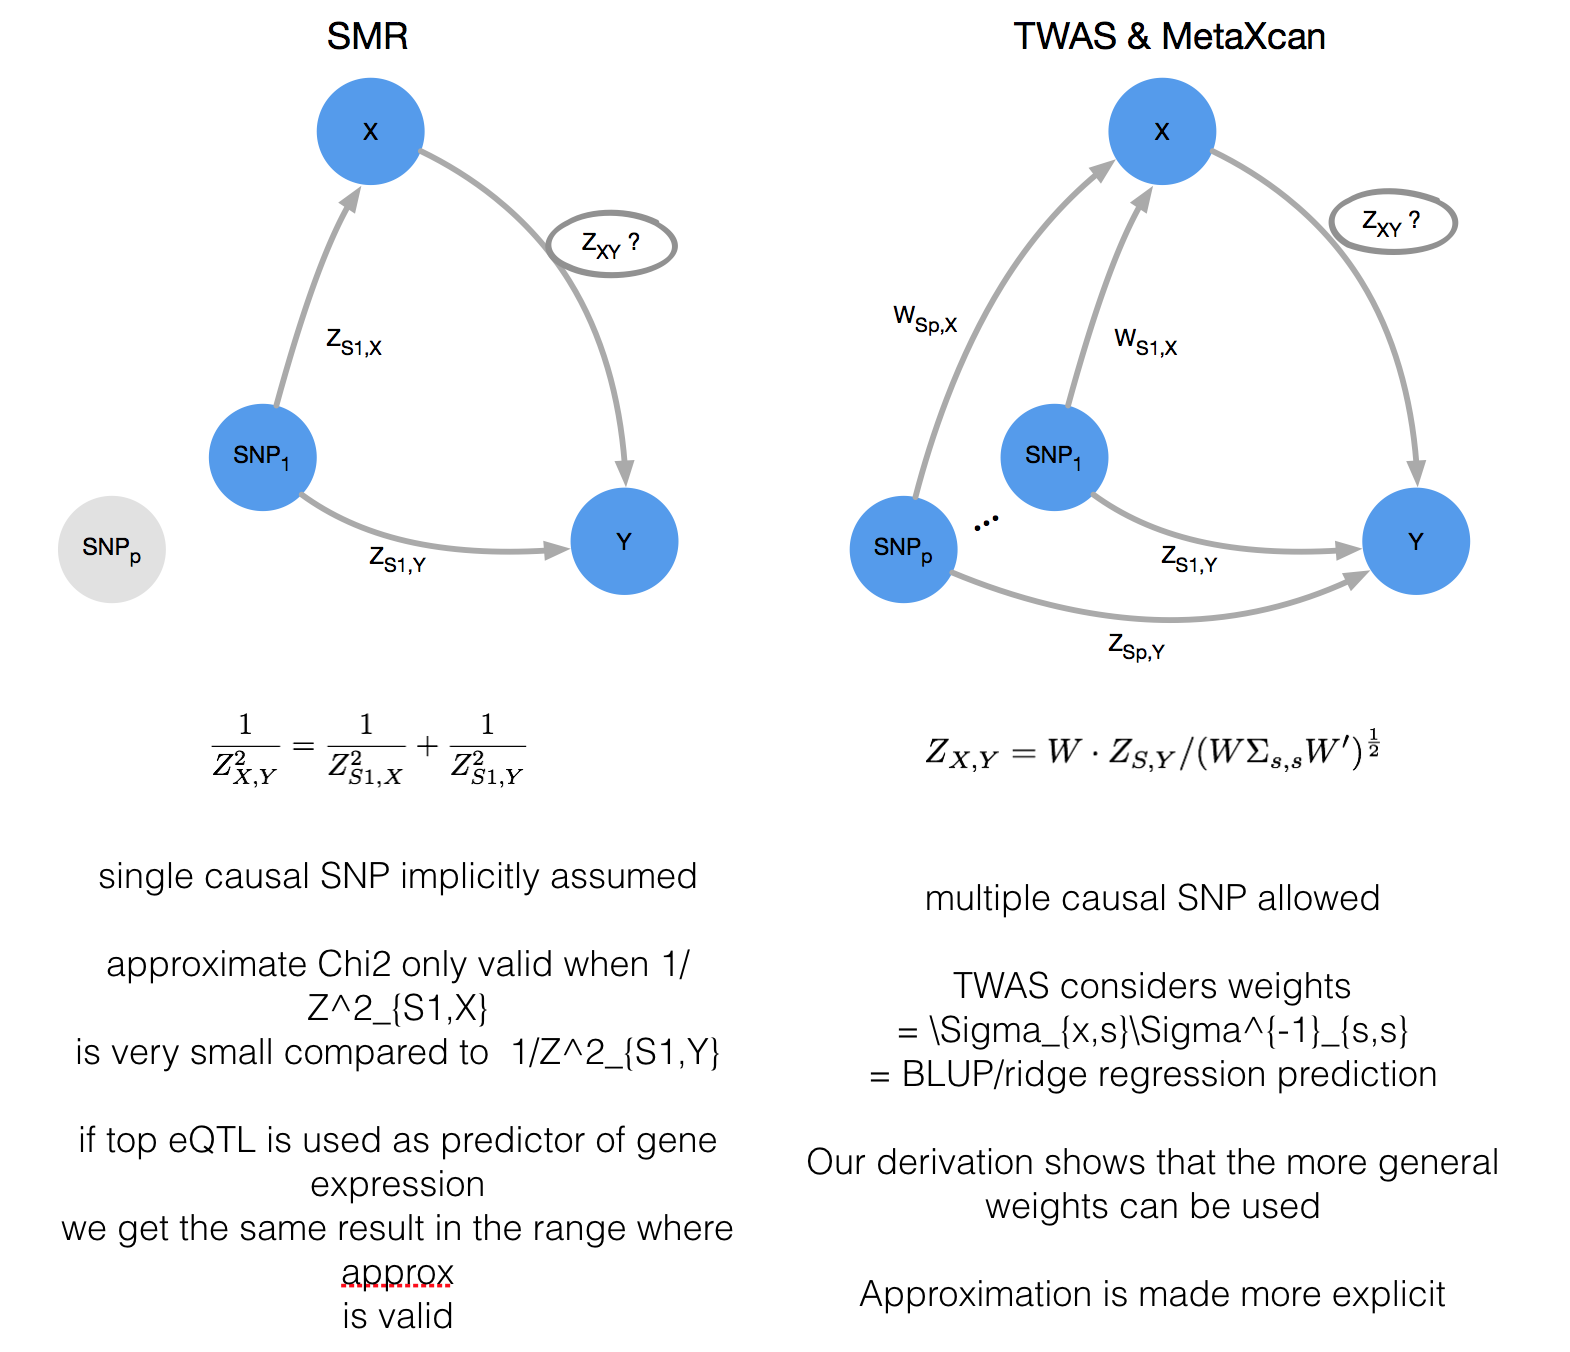
\includegraphics[width=\textwidth]{plots/MetaXcan-vs-SMR-TWAS.png}
\caption{CAPTION. \hl{TODO generate better figures}}
\label{fig:MetaXCan-vs-SMR-TWAS}
\end{figure}


Yang et al have proposed SMR \cite{SMR}, a summary data based Mendelian randomization that integrates eQTL results to determine target genes of complex trait-associated GWAS loci. 

They derive an approximate chi-square statistic (Eq 5 in SMR) for the mediating effect of the target gene expression on the phenotype. We write the expression in terms of the inverse of the statistic that is easier to interpret. 

\begin{equation}
\frac{1}{T_\text{SMR}} = \frac{1}{Z^2_\text{eqtl}} + \frac{1}{Z^2_\text{GWAS}}  
\label{eq5-SMR}
\end{equation}

where $T_{SMR}=(\text{effect size} / \text{standard error})^2$ , $Z_\text{eqtl}$ is the Z score (=\text{effect size} / \text{standard error}) of the association between SNP and gene expression, and $Z_\text{GWAS}$ is the Z score of the association between SNP and trait. 

Thus the inverse of the square of the Wald statistic derived by Yang et al is the sum of two inverse $\chi^2$ (Z is asymptotically normally  Z2 is chisquare  1/Z2 is inverse chisquare). 

We know that the sum of two inverse $\chi^2$ random variables does not yield a $\chi^2$, so that there are additional assumptions that need to be made. Since each term is inverse  $\chi^2$, for the sum to be inverse  $\chi^2$, one of the two terms must be negligible compared to the other. SMR assumes that the eQTL effect is strong, i.e. when the first term on the RHS is small. Under this assumption the $T_{SMR}$ is approximately $\chi^2$.

% \textbf{Top eQTL driven SMR.} 
SMR is applied transcriptome wide using the top eQTL for each gene. If we use the top eQTL as the sole predictor of gene expression in PrediXcan/MetaXcan, the association statistic is equal to 1/Z2(GWAS). Thus under the assumption of strong eQTL effect, SMR is equivalent to MetaXcan using top eQTL to predict expression level of the (potential) target gene.

SMR will work well when there is a single variant that affects expression levels and through them alters the phenotype. In this case, an advantage of SMR over MetaXcan is that it incorporates uncertainty in the eQTL association $\frac{1}{Z^2_\text{eqtl}}$. However, in the range where the statistic $T_\text{SMR}$ is approximately correct, the difference between MetaXcan and SMR results is also negligible. Extension of MetaXcan that takes into account the uncertainty in the prediction models will be ideal.

% Top GWAS driven SMR
% It is possible to use the top GWAS SNP in each GWAS locus and evaluate the SMR statistic for all genes in the vicinity of the SNP. The difference with the eQTL driven SMR is the number of multiple testing to account for. This approach may make more sense if the GWAS is much better powered than the eQTL study. SMR assumption would not hold in this case. 

\subsubsection*{Comparison with TWAS (Gusev/Pasaniuc NG)}

Gusev et al have proposed a method comparable to MetaXcan that is based only on summary statistics. This method, called Transcriptome-Wide Association Study (TWAS), imputes the SNP level z-scores into gene level z-scores using the method Pasaniuc and others have published \cite{Pasaniuc2014}. This approach is equivalent to predicting expression levels using BLUP/Ridge Regression, which has been shown to be suboptimal \cite{Wheeler2016}. This is due to the fact that the local architecture of gene expression traits is sparse so that highly polygenic models underperform more sparse prediction models such as LASSO or Elastic Net with mixing parameters 0.5 or greater.

\subsubsection*{Prediction models across human tissues}

Using the release version 6p (dbGaP Accession phs000424.v6.p1) from GTEx, we have trained prediction models for expression levels of 44 human tissues with a total of 1,091,787 gene tissue pairs. Among these 203,494 yielded prediction models with cross validated q value $<$ 0.05 (FDR computed among each tissue models), which were saved into the Predictdb database and used for subsequent analysis.

We use SNPs within 1Mb upstream of the TSS and 1Mb downstream of the TES. We use elastic net with a mixing parameter of 0.5, a multivariate linear model estimated via penalized maximum likelihood. As reported in \cite{Gamazon2015,Wheeler2016} overall performance does not vary for a range of values of the mixing parameter except when the model becomes very close to ridge regression (fully polygenic). Based on this we chose to use elastic net with 0.5 as mixing parameter, which will be more robust to low qualify genotype or imputation.

%In addition to the 44 GTEx tissue models, we use the whole blood model trained with 922 samples from the Depression and Genes Network cohort and a derived expression trait that represents a component common across multiple tissues.

Supplementary Table 1: list of tissues, sample sizes, summary R2, \# with qval < 0.05, \# total attempted training, \# total successful models.

\subsubsection*{Catalog of the phenotypic consequences of gene regulation}

Next we downloaded summary statistics of meta analysis of 113 phenotypes (encompassing xxx main phenotypes) from 16 consortia. The full list of consortia and phenotypes is shown in Supplementary Table 2. We computed association between these phenotypes and the predicted expression levels in 44 human tissues using elastic net models described in the previous section and a whole blood model. \hl{TODO Alvaro: create top eQTL model using the Blood eqtl summary data and run metaxcan. this should serve as an additional training set replication for whole blood.}

To facilitate query of the results, we created a web application that allows filtering the results by gene, phenotype, tissue, p value, and prediction performance (gene2pheno.org).
For each trait we assigned ontology terms from EFO and HPO. 

Supplementary Table 2: List of consortia and phenotypes for which gene level association are available. Gene/tissue pair results were considered significant when p-value<0.05/total number of gene/tissue pairs tested (which ranged from xxe-6 - xxe-6).

Manhattan and qqplots for each phenotype (all tissue results combined) can be found in Supplementary Figure xx.

Mostly genome-wide significant genes tend to cluster around SNP level genome-wide significant loci or sub-genome wide significant loci. Because of the reduction in multiple testing or an increase in power because it takes into account of the combined effects of multiple variants, sub-genome-wide significant genes can become gw significant in MetaXcan. \hl{Alvaro TODO: find examples. Do we find examples where MetaXcan p values are more significant than GWAS pvalues? I am guessing not but please check.}

Results of MetaXcan tend to be more significant as R2 goes up, i.e. the genetic component of expression is larger. The trend is seen both when results are averaged across all tissues for a given phenotype or across all phenotypes for a given tissue. Representative phenotypes were chosen. Using squared zscores or abs zscores did not change results much. 

\begin{figure}
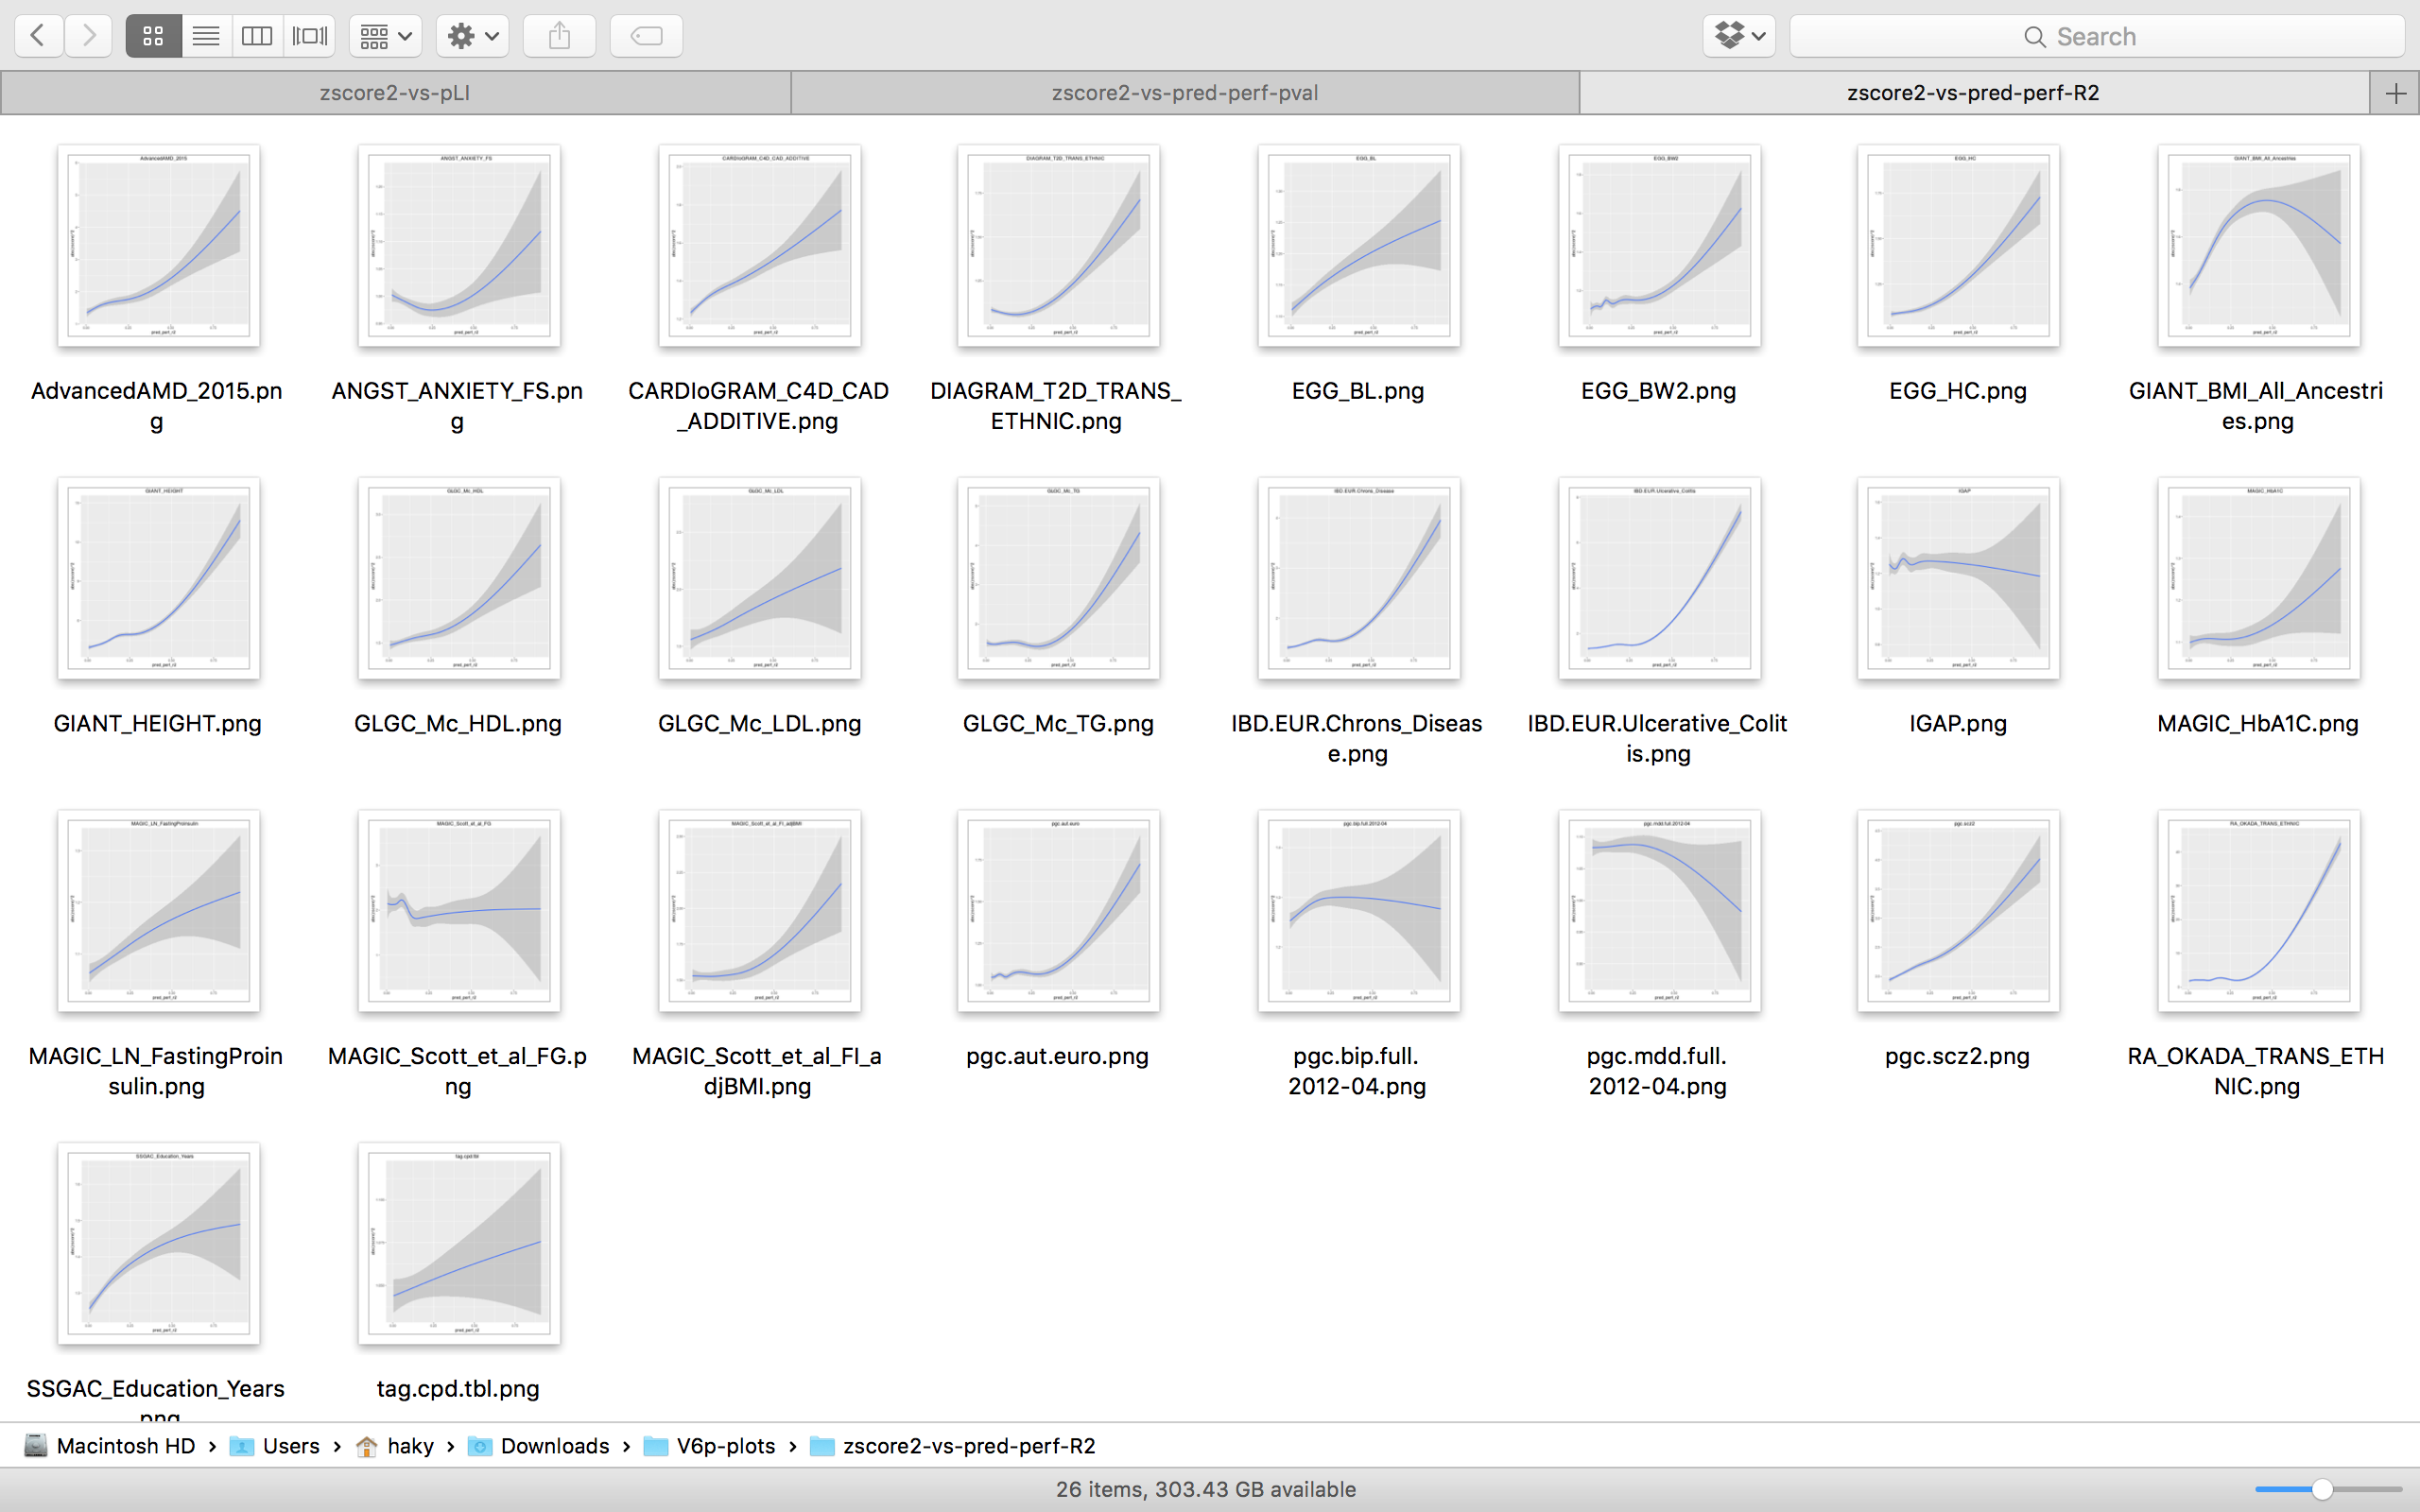
\includegraphics[width=\textwidth]{plots/Fig6a-zscore2-vs-pred-perf-R2-by-phenotype.png}
\caption{zscore2 vs predicted performance R2 by phenotype \hl{TODO generate better figures, move these large figures to supplementary. Combine all four Z2 vs R2 and pppval into one figure.}}
\label{fig:zscore2-R2-pheno}
\end{figure}

\begin{figure}
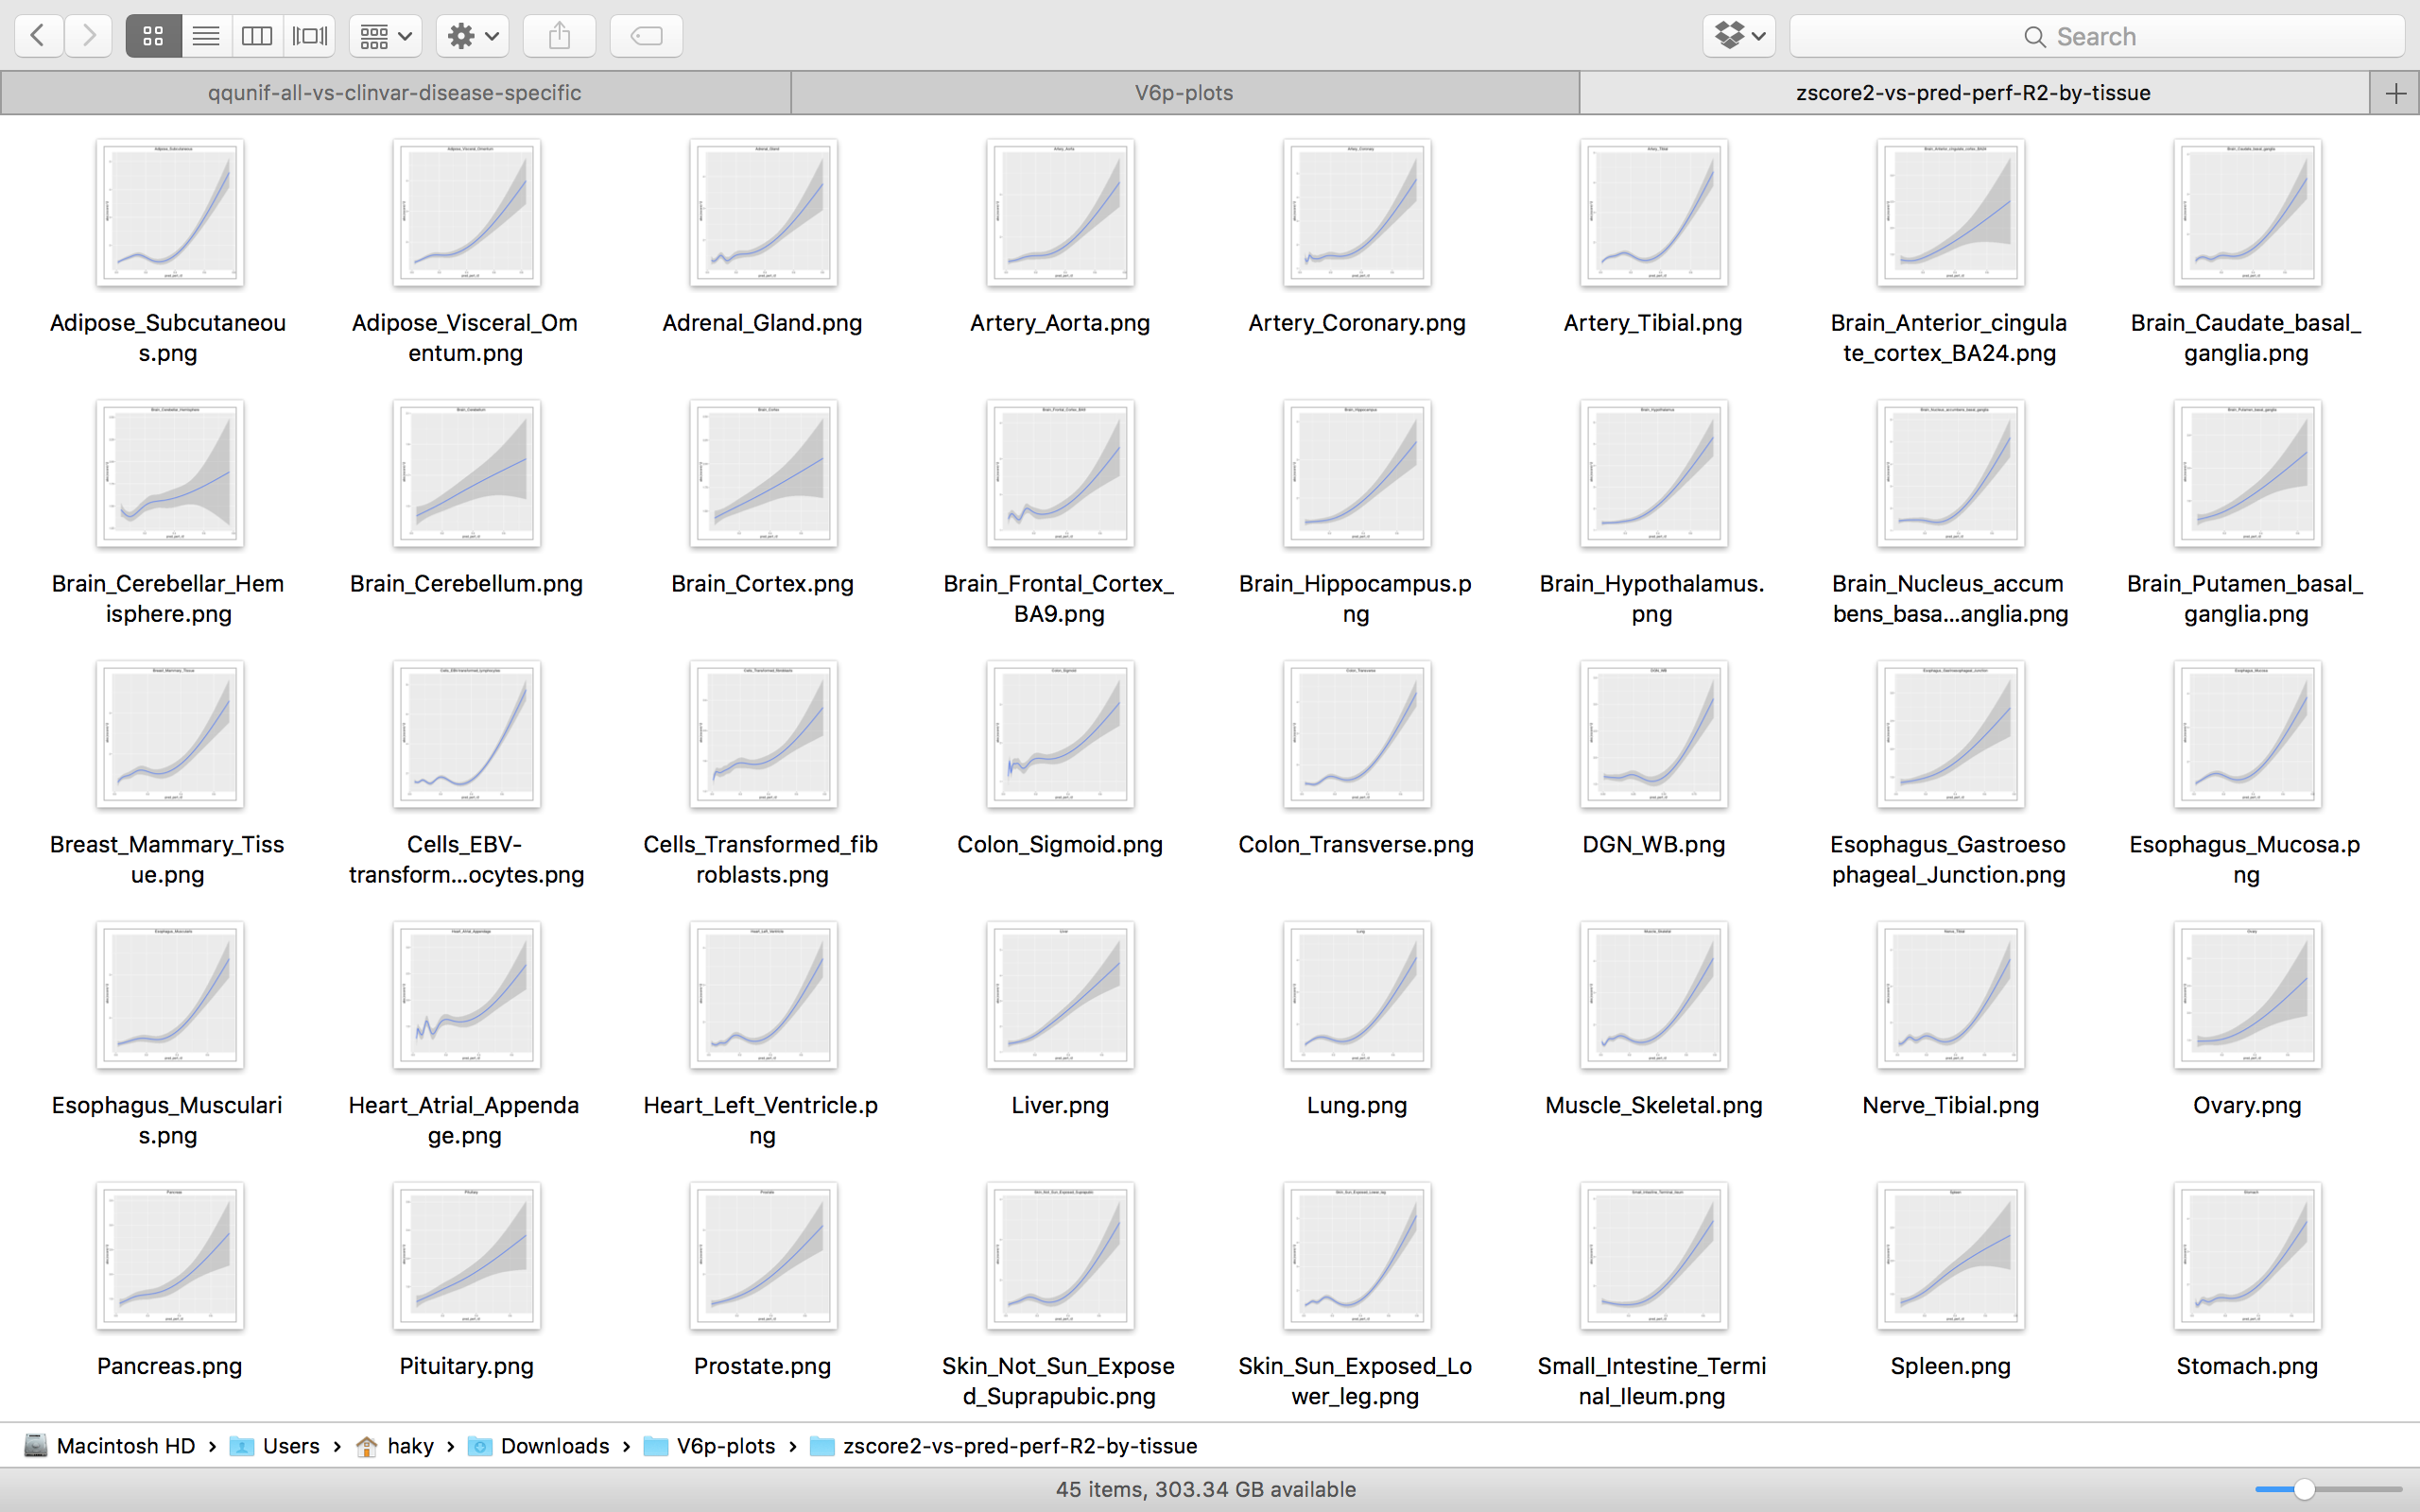
\includegraphics[width=\textwidth]{plots/Fig6b-zscore2-vs-pred-perf-R2-by-tissue.png}
\caption{zscore2 vs predicted performance R2 by tissue \hl{TODO generate better figures, move these large figures to supplementary. Combine all four Z2 vs R2 and pppval into one figure.}}
\label{fig:zscore2-R2-tissue}
\end{figure}

Similarly, results of MetaXcan tend to be more significant as prediction p values are more significant. The trend is seen both when results are averaged across all tissues for a given phenotype or across all phenotypes for a given tissue. Representative phenotypes were chosen. Using squared zscores or abs zscores did not change results much. 

\begin{figure}
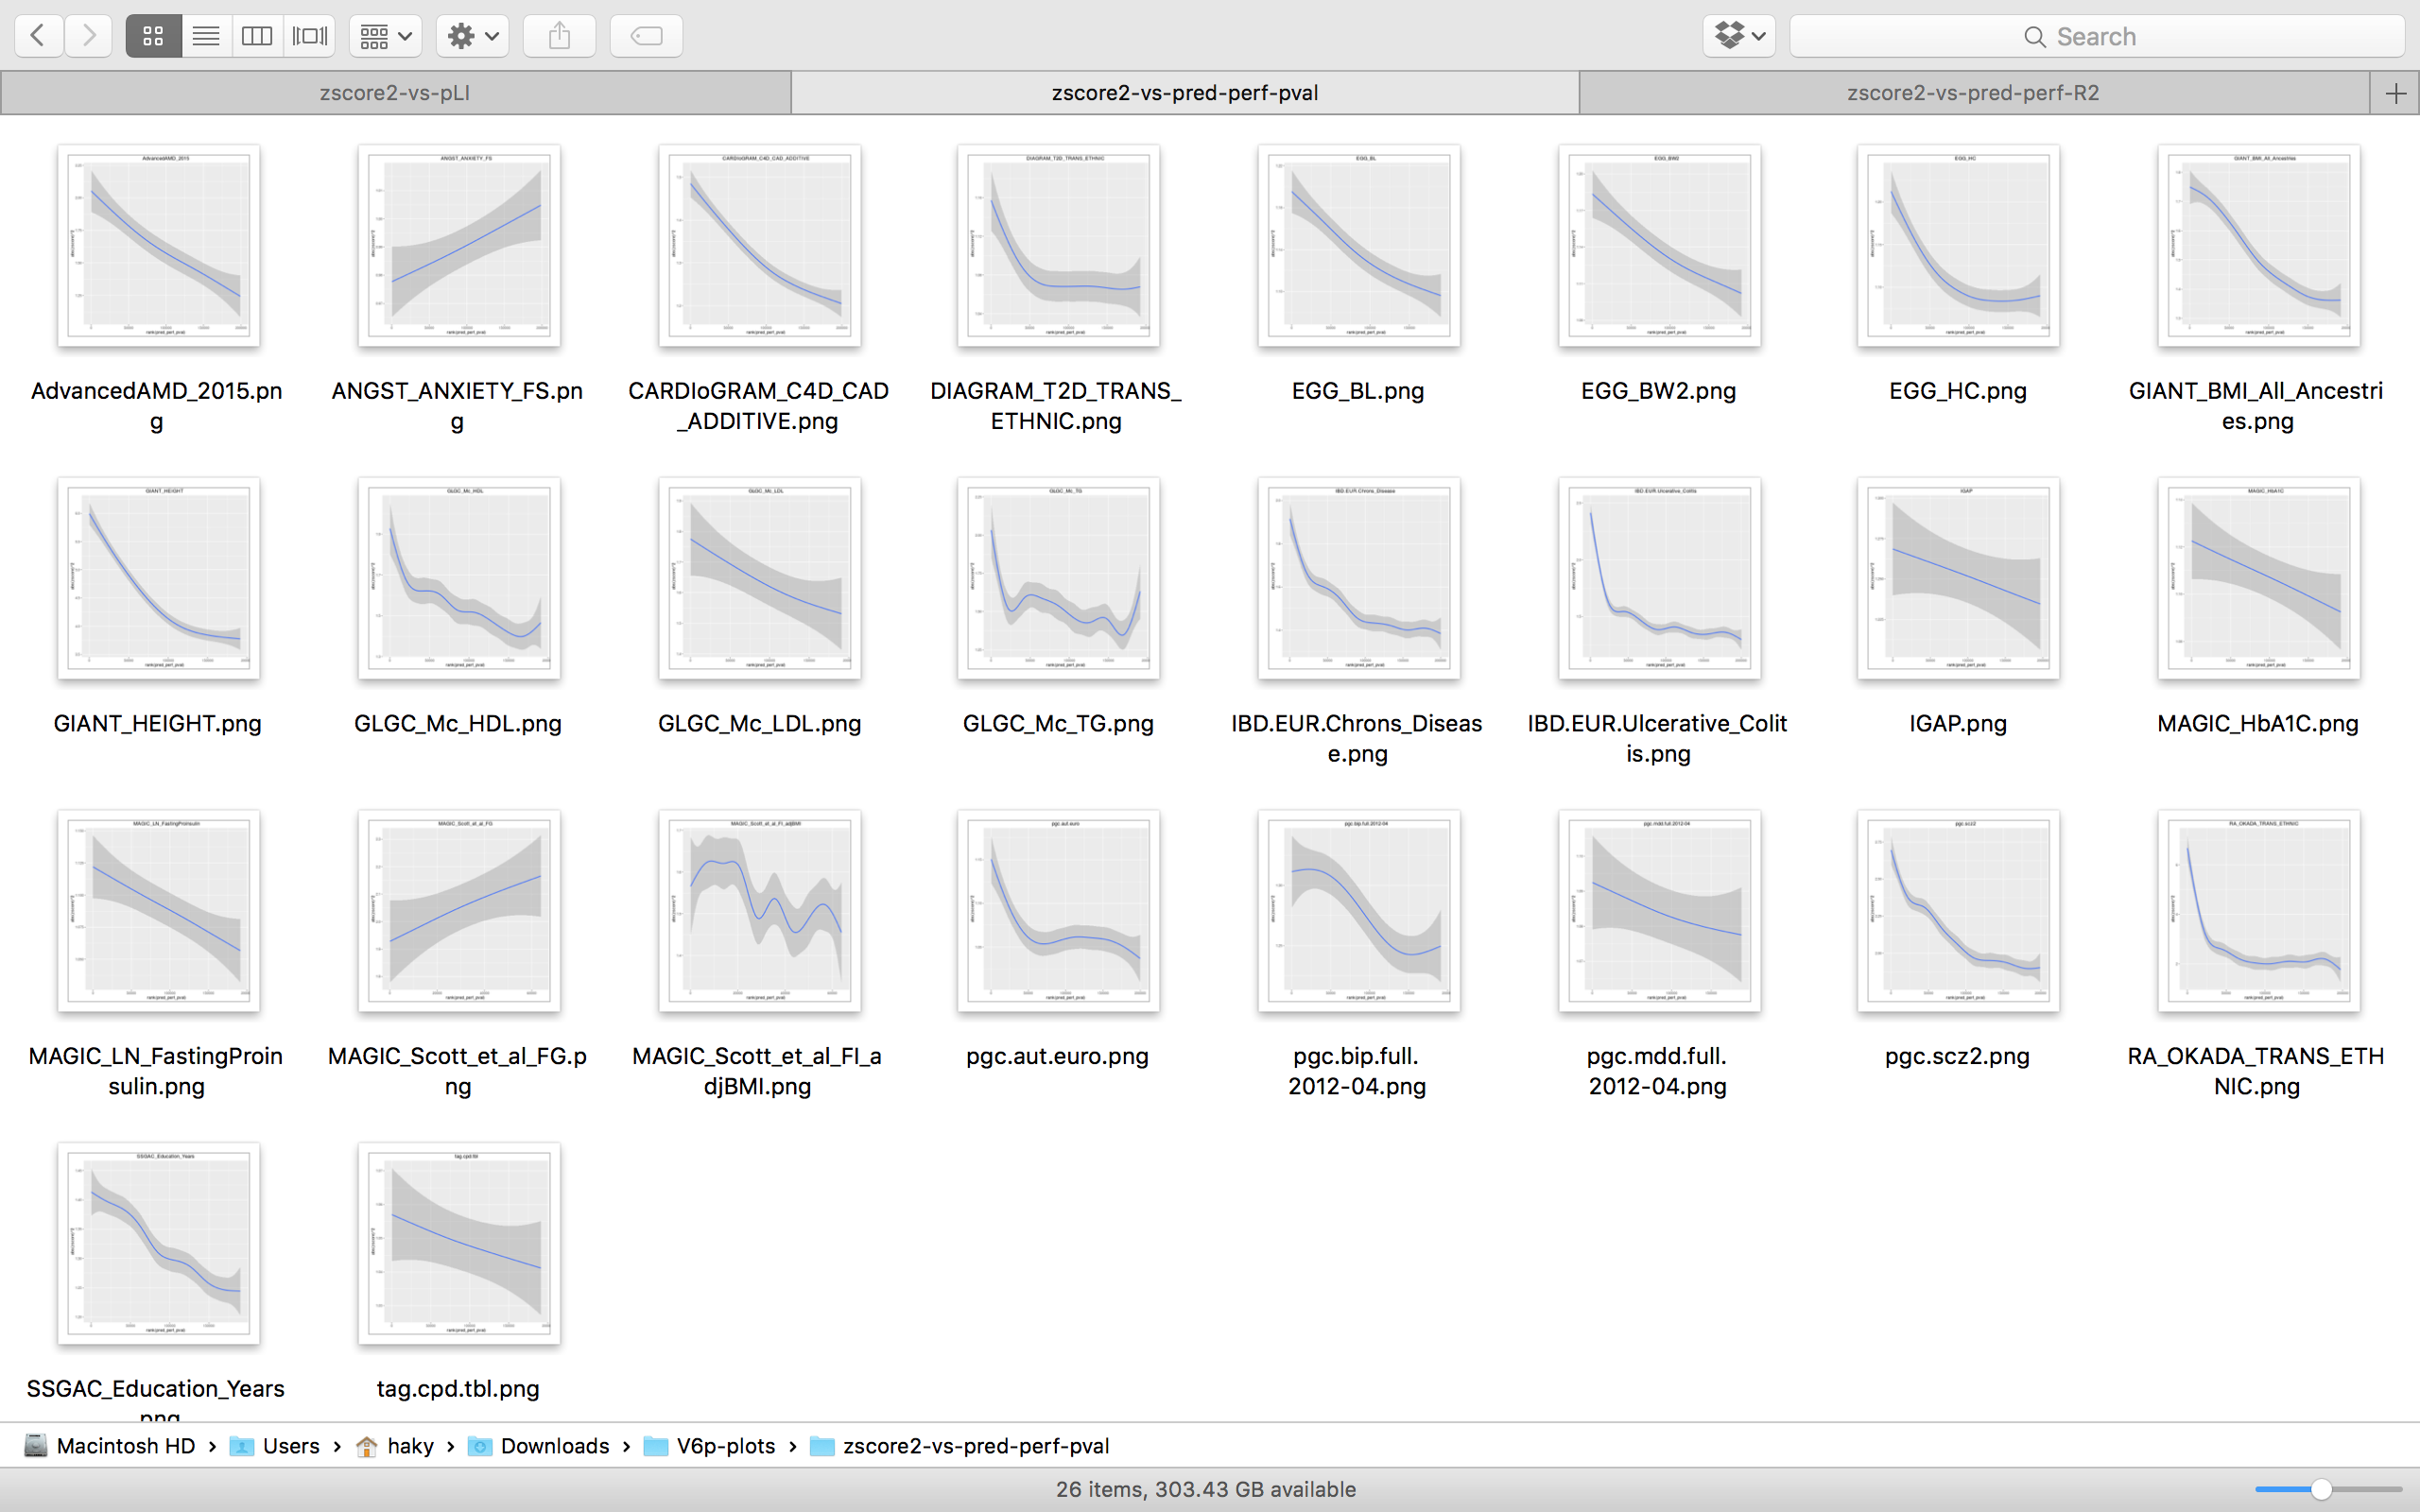
\includegraphics[width=\textwidth]{plots/Fig7a-zscore2-vs-pred-perf-pval-by-phenotype.png}
\caption{zscore2 vs predicted performance pval by phenotype \hl{TODO generate better figures}}
\label{fig:zscore2-pval-pheno}
\end{figure}

\begin{figure}
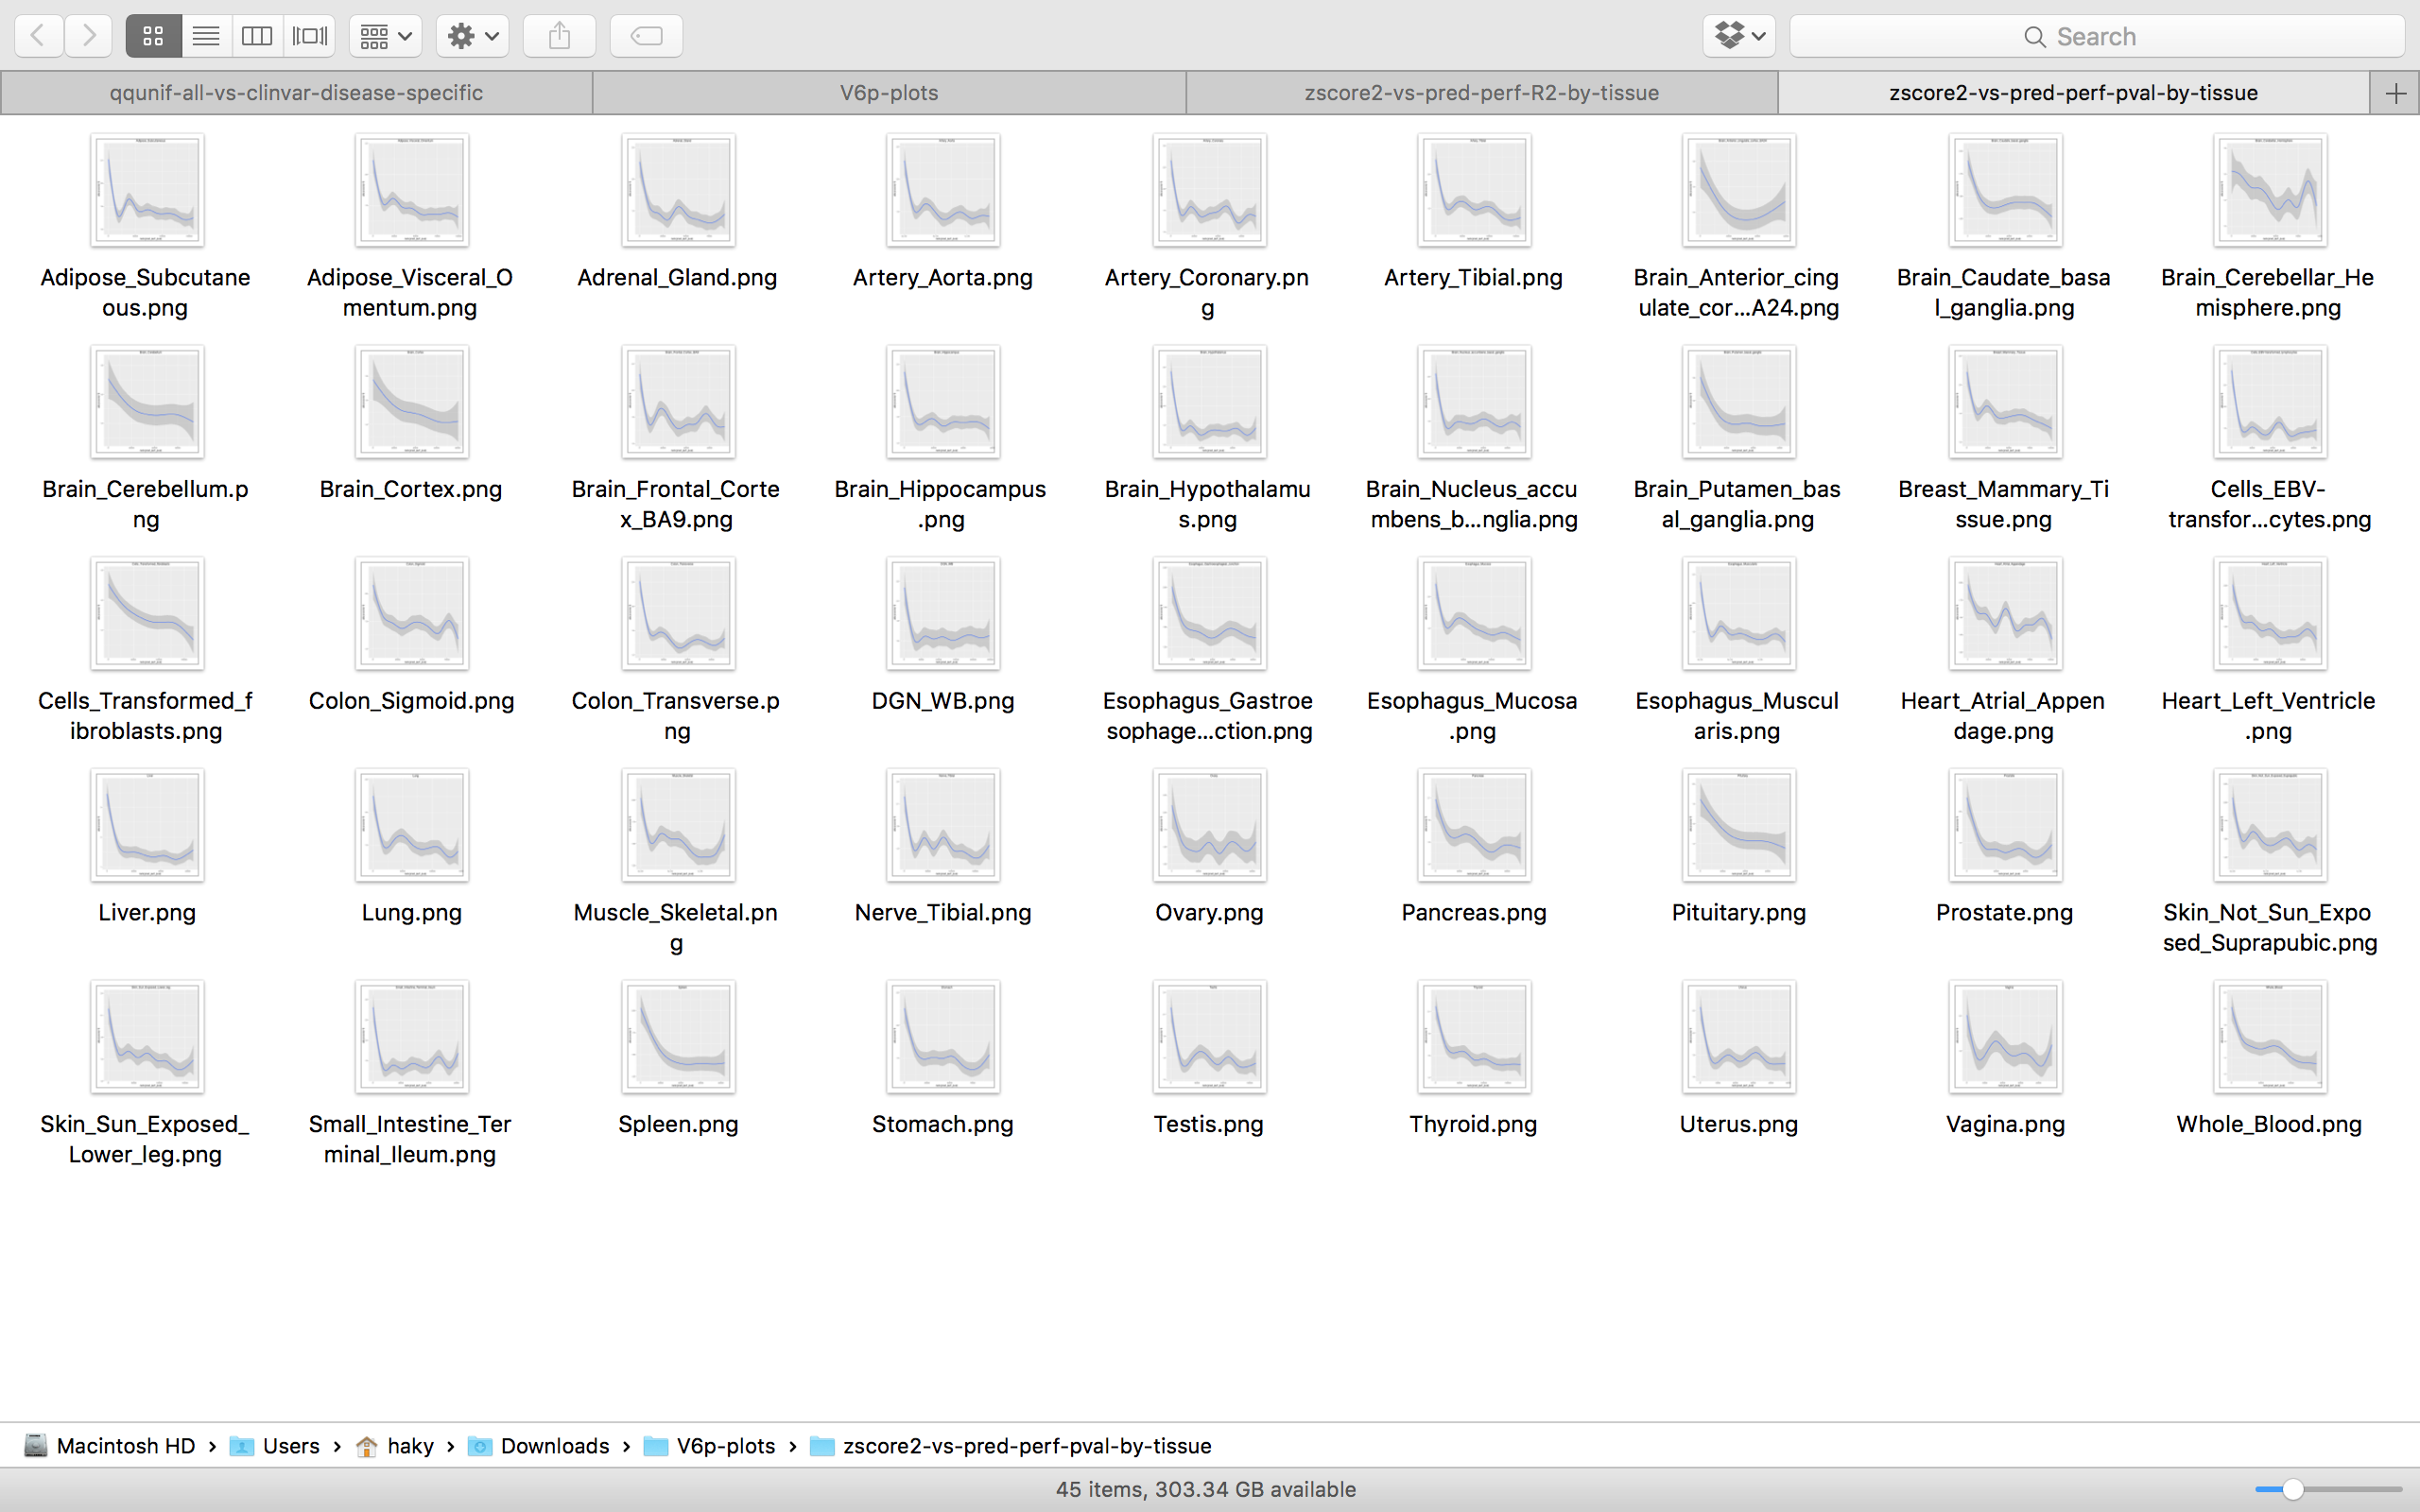
\includegraphics[width=\textwidth]{plots/Fig7b-zscore2-vs-pred-perf-pval-by-tissue.png}
\caption{zscore2 vs predicted performance pval by tissue \hl{TODO generate better figures}}
\label{fig:zscore2-pval-tissue}
\end{figure}





% \subsubsection*{Enrichment of loss of function mutation intolerant genes}

% There seems to be a deflation of significance among LoF intolerant genes (pLI>0.9) in disease phenotypes whereas for biomarkers such as LDL, TG, FG, FI there seems to be an inflation. Not sure what to make of this. %https://www.dropbox.com/sh/74a5b4956xywtbk/AADzF07pf6yO96QRcwWaNU1ja?dl=0 

\subsubsection*{Enrichment of genes in ClinVar}

Genes implicated in ClinVar to obesity, rheumatoid arthritis, diabetes, Alzheimer's, Crohn's disease, ulcerative colitis, age-related macular degeneration, and autism show inflated significance among metaxcan association results for corresponding diseases. Schizophrenia genes (20 available) do not show any inflation (probably a limitation of the ClinVar database).
\begin{figure}
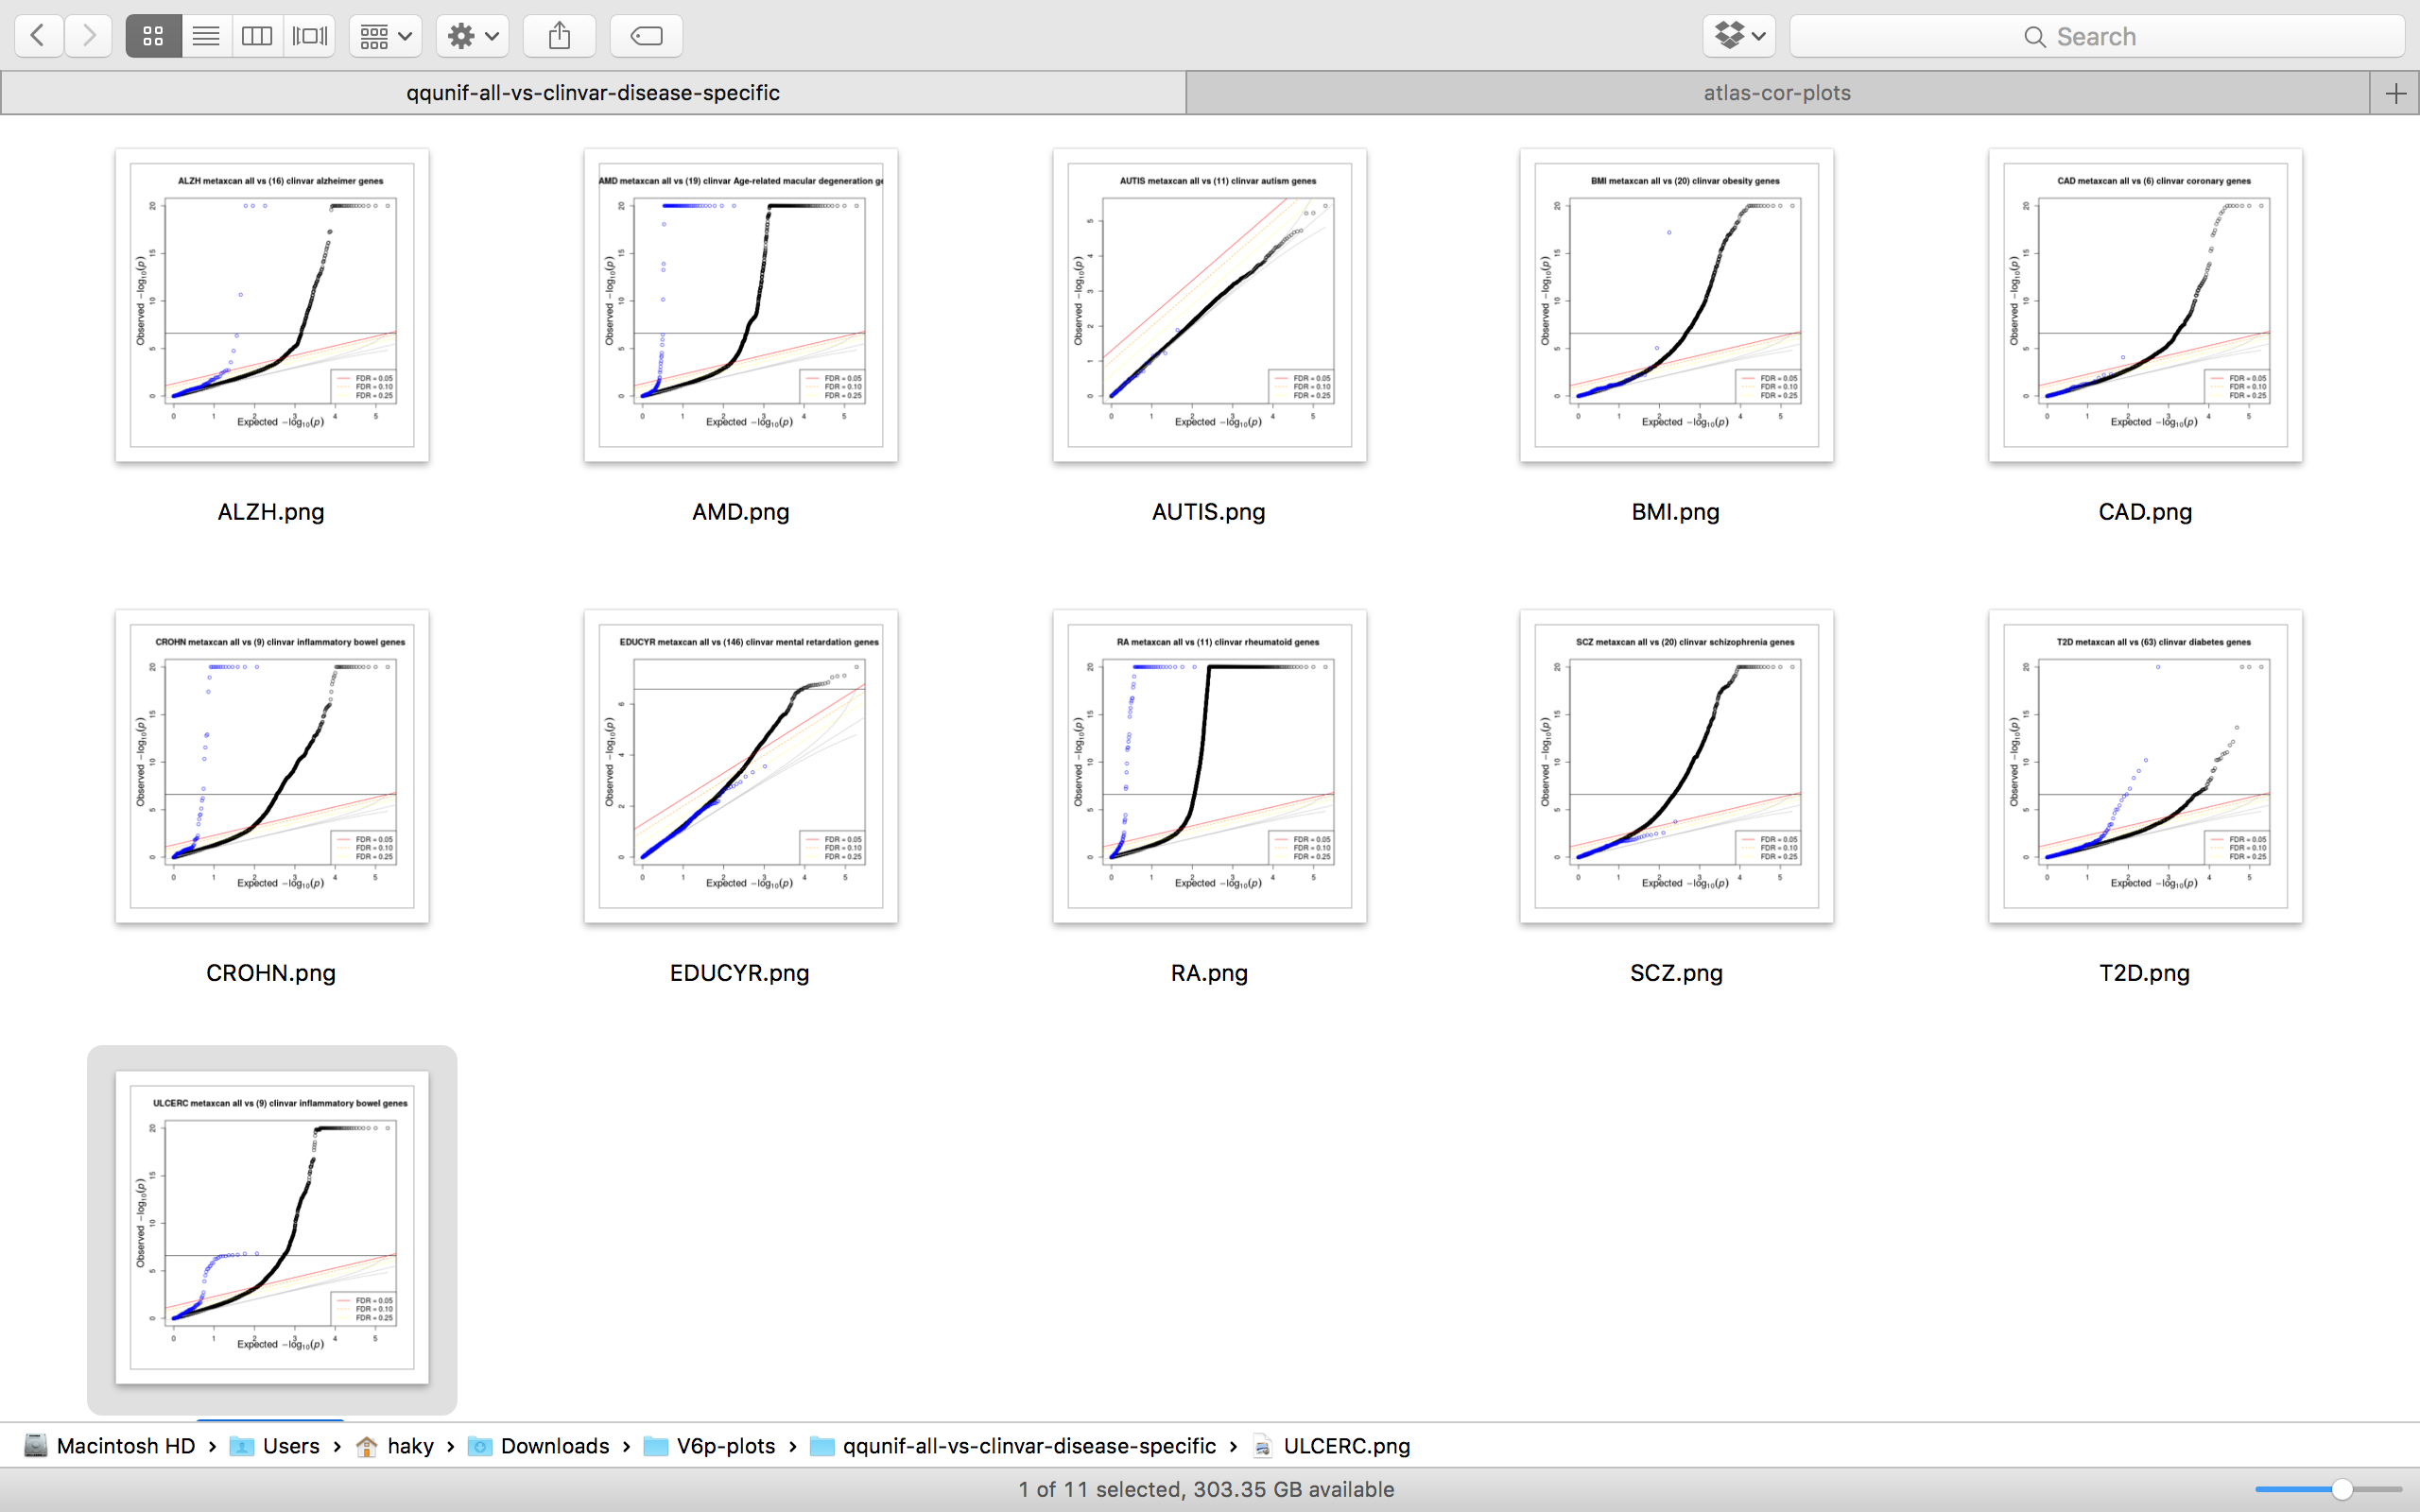
\includegraphics[width=\textwidth]{plots/Fig8-clinvar-vs-metaxcan.png}
\caption{ClinVar genes enriched among significant metaxcan genes for most diseases we tested except for schizophrenia. \hl{TODO generate better figures}}
\label{fig:clinvar}
\end{figure}

\subsubsection*{qqplot comparing all pvals vs tissue specific pvals}

 When comparing p-value distributions for different tissues, we were expecting to find that tissues relevant to the disease would show up as more significant. We find this to be the case for coronary artery disease: the tissues with most significant genes were Artery tissues (coronary, tibial, and aorta) and liver. Also LDL cholesterol associated genes showed enrichment of genes predicted in liver. However that was not the case for HDL and TG, for which whole blood models were most enriched among top results. In T2D, muscle models depart the most from the reference distribution. But this is due to only a handful of genes. Also TCF7L2, a positive control gene for T2D, only shows significant association in aortic artery.

\subsubsection*{What is the difference between regions with multiple target genes and single target genes?}
\subsubsection*{What is the difference between regions with genes significant across multiple tissues vs single tissues?}
\subsubsection*{how to distinguish causal vs passenger association?}

\subsubsection*{Regulation may not always be identifiable in the tissue of action}

There is value in looking at the results across all tissues even though the causal mechanism that alters disease risk may not happen in all tissues, the regulation may be detectable in other tissues.

For example, rs11206510 and rs2479394 were shown to be eQTL in VAF (Visceral Abdominal Fat) in the STARLET study and a study with morbidly obese patients (Greenawalt, Genome Res 2011). 

However in GTEX rs11206510 was associated with PCSK9 only at p=0.035, which in the context of genome wide study with multiple testings would not reach significance. 


However in GTEx, we find that the regulation of PCSK9 is much more active in tibial nerve. It is unlikely that tibial nerve is the tissue of action of cardio-metabolic traits. (p=1e-14 and 1e-6)

Conditions of sample treatment (extraction, treatment) and demographic variables results in making tibial nerve the most conducive environment to detect the link between these variants and PCSK9.

\begin{figure}
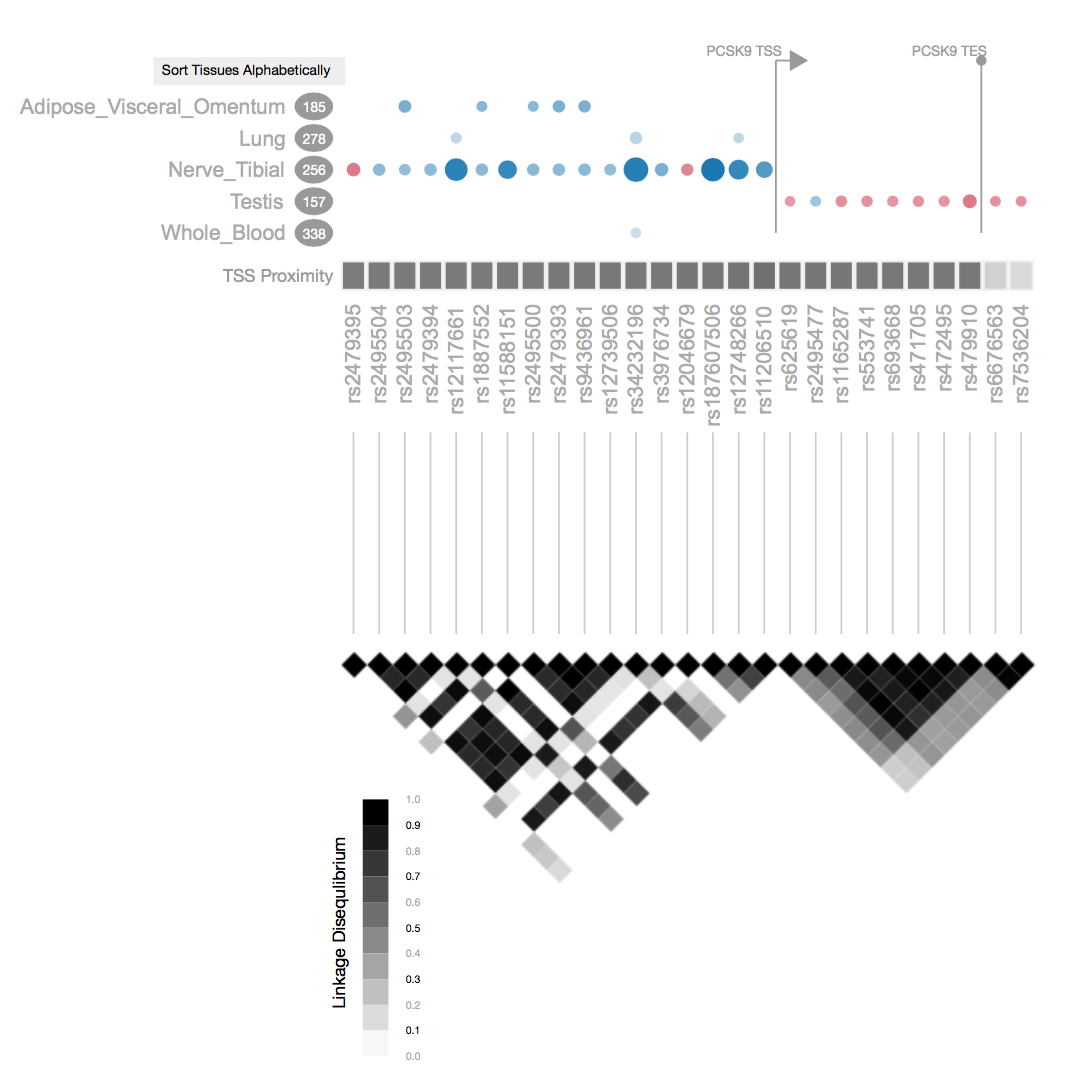
\includegraphics[width=\textwidth]{plots/Fig10-PCSK9-eQTL-Visualizer.png}
\caption{PCSK9 most actively regulated in Tibial Nerve in GTEx. \hl{TODO generate better figures}}
\label{fig:PCSK9-eqtl}
\end{figure}


\subsubsection*{Results across all tissues as replicated experiments}

Since it has been reported that a large portion of cis regulation is shared across tissues we hypothesize that gene level associations can be detected using tissues that are not necessarily the tissue of action of the disease. Also the complexity of gene regulation and perhaps environmental state dependence of regulatory processes our models may be missing some of the associations because they are based on a one-time snapshot of the transcriptome averaged over many cells. Our results suggest that expanding our analysis to tissues other than the ones we expect to be involved in the phenotype of interest increases our ability to identify disease relevant genes. 

\subsubsection*{Correlation between phenotypes}
For a given tissue, we computed the correlation between the zscores from different phenotypes. The correlation is consistent with the results reported by Bulik-Sullivan et al. 

\begin{figure}
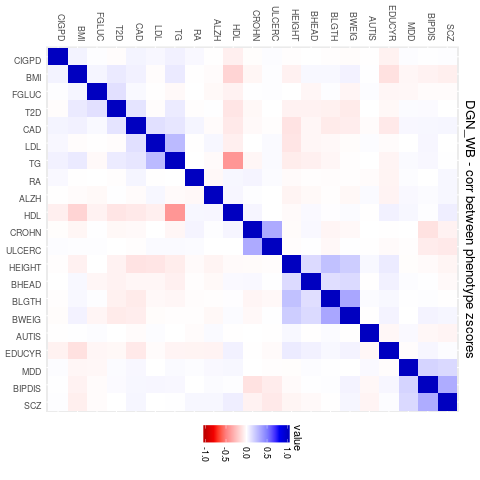
\includegraphics[width=\textwidth]{plots/Fig9-corr-traits-DGN_WB.png}
\caption{Correlation between traits. \hl{TODO generate better figures}}
\label{fig:corr-traits}
\end{figure}




\subsubsection*{Software}

We make our software publicly available on a GitHub repository: \url{https://github.com/hakyimlab/MetaXcan}. Instructions for obtaining the weights and covariances for different tissues can be found there. A short working example can be found on the GitHub page; more extensive documentation can be found on the project's wiki page.

% For ease of use, we have developed a desktop GUI application. We have also developed a web-based version to further simplify the use of the method, available at: \url{http://hakyimlab.org/metaxcan/})

%\begin{figure}
%\includegraphics[width=0.6\textwidth]{plots/gui.png}
%\caption{ GUI application running in a local environment. }
%\label{fig:gui}
%\end{figure}
 
%\begin{figure}
%\includegraphics[width=0.6\textwidth]{plots/WebAppExample.png}
%\caption{ Web Based version, available at \url{http://hakyimlab.org/metaxcan/}}
%\label{fig:webapp}
%\end{figure}

\section*{Discussion}

Here we present MetaXcan, a scalable, accurate, and efficient method for integrating reference transcriptome studies to learn about the biology of complex traits and diseases. Our method extends PrediXcan, which maps genes to phenotypes by testing the mediating effects of gene expression levels. This is implemented by predicting gene expression levels  and correlating these traits with phenotypes. MetaXcan is a shortcut that uses SNP-level association results and combines them to reproduce the results of PrediXcan, without the need to use individual level data.

MetaXcan shares most of the benefits of PrediXcan: a) it directly tests the regulatory mechanism through which genetic variants affect phenotype; b) it provides gene-level results which are better functionally characterized than genetic variants, easier to validate within model systems, and carry a smaller multiple testing burden; c) the direction of the effects are known, facilitating identification of therapeutic targets; d) reverse causality is largely avoided since predicted expression levels are based on germline variation, which are not affected by onset of disease; e) it can be systematically applied to existing GWAS studies; f) tissue-specific analysis can be performed using all the models we have made available through PredictDB (\url{http://predictdb.org}).

The difference between the reference sets (used to estimate LD and allele frequencies) and study set (used to compute GWAS/meta analysis summary statistics) is the main cause of the small differences between MetaXcan and PrediXcan results. We have shown here that even when the populations are quite different, the concordance is very high. Thus, MetaXcan is robust to ancestral differences between study and reference sets.

Even though the method was derived with linear regression in mind, in relatively well balanced (less than 3 to 1 ratio between groups) case-control designs, the approximation generates results that are in almost full concordance with exact results generated with PrediXcan and logistic regression.

Methods similar in spirit to PrediXcan have been reported \cite{Gusev2016}. Gusev et al also propose a method comparable to MetaXcan that is based only on summary statistics. Their method, called Transcriptome-Wide Association Study (TWAS), imputes the SNP level z-scores into gene level z-scores using ImpG, a method proposed by Pasaniuc and others \cite{Pasaniuc2014}. This approach is equivalent to predicting expression levels using BLUP/Ridge Regression, which has been shown to be suboptimal for prediction. This is due to the fact that the local architecture of gene expression traits is sparse so that highly polygenic models underperform more sparse prediction models such as LASSO or Elastic Net with mixing parameters 0.5 or greater \cite{Wheeler2016}.

In contrast, MetaXcan is not restricted to one imputation or prediction scheme. It
infer the results of PrediXcan using summary statistics through an analytic formula. Thus it can be applied to any linear models based on SNP data. For example, given the LD we are able to "predict" structural variation or more complex genetic variation as a linear function of SNP data. MetaXcan allows us to infer the assocation between these variants and complex traits using existing publicly available summary statistics.

In summary, we present an accurate and computationally efficient gene-level association method that integrates functional information from reference transcriptome dataset into GWAS and large scale meta-analysis results to inform the biology of complex traits.

We show that MetaXcan includes other state of the art methods such as TWAS and SMR as special cases when the appropriate prediction model is selected.

Furthermore, we train prediction models for 44 human tissue expression levels from GTEx and apply to 117 phenotypes with meta analysis results publicly available from 16 large consortia. 

As expected, better predicted genes (larger heritable component or more significant predictions) are more likely to be identified as associated with complex traits. We also find that for the disease genes we have tested ClinVar genes are highly enriched.

Due to the large shared regulation across tissues, we found that examining results in tissues that are not traditionally considered relevant for the disease of interest increase our ability to identify disease genes.


\section*{Methods}

\subsection*{Derivation of MetaXcan Formula}

The goal of MetaXcan is to infer the results of PrediXcan using only GWAS summary statistics. Individual level data are not needed for this algorithm. We will define some notations for the derivation of the analytic expressions of MetaXcan.

\subsubsection*{Notation and Preliminaries}

$Y$ is the $n$-dimensional vector of phenotype for individuals $i=1,n$.\\
$X_l$ is the allelic dosage for SNP $l$.\\
$T_g$ is the predicted expression (or estimated GREx, genetically regulated expression).\\
We model the phenotype as linear functions of $X_l$ and $T_g$
\begin{align*}
Y &= X_l \beta_l + \eta\\
Y &= T_g \gamma_g + \epsilon,
\end{align*}
where $\hat\gamma_g$ and $\hat\beta_l$ are the estimated regression coefficients of $Y$ regressed on $T_g$ and $X_l$, respectively. $\hat\gamma_g$ is the result (effect size for gene $g$) we get from PrediXcan whereas $\hat\beta_l$ is the result from a GWAS for SNP $l$.

We will denote as Var and Cov the operators that computes the sample variance and covariances, i.e. Var($Y$) = $\sum_{i=1,n} (Y_i - \bar{Y})^2/n$ with $\bar{Y} = \sum_{i=1,n} Y_i / n$\\
$\hat\sigma^2_l = $  Var$(X_l)$\\
$\hat\sigma^2_g = $  Var$(T_g)$\\
$\hat\sigma^2_Y = $  Var$(Y)$\\
$\Gamma_g = \mathbf{(X-\bar{X})'(X-\bar{X})}/n$,\\ 
 where  $\mathbf{X'}$ is the $n \times p$ matrix of SNP data and $\mathbf{\bar{X}}$ is a $n \times p$ matrix where column $l$ has the column mean of $\mathbf{X}_l$ ($p$ being the number of SNPS in the  model for gene $g$).\\
% * <jason.matthew.torres@gmail.com> 2015-11-11T17:58:12.506Z:
%
% Can you make it more explicit, where the g fits into the covariance formula. I'm not sure if readers will readily appreciate that this refers to the convariance of SNP predictors for gene g. 
%
% ^.

With this notation, our goal is to infer PrediXcan results ($\hat\gamma_g$ and its standard error) using only GWAS results ($\beta_l$ and se), estimated variances of SNPs 
($\hat\sigma^2_l$), covariances between SNPs in each gene model ($\Gamma_g$), and prediction model weights $w_{lg}$.\\

\textbf{Input:}  $\beta_l$, se($\beta_l$), $\hat\sigma^2_l$, $\Gamma_g$, $w_{lg}$.
\textbf{Output:} 
$\hat\gamma_g$, se($\hat\gamma_g$).\\
%From these the Zscore ($Z = \hat\gamma_g$/ se($\hat\gamma_g$)) and p value ($p$= 2 pnorm($-|Z|$) ) can be computed.

Next we list the properties and definitions used in the derivation: 
\begin{equation}
\hat\gamma_g = \frac{ \text{Cov}(T_g,Y) }{ \text{Var}(T_g)}  =  \frac{ \text{Cov}(T_g,Y) }{ \hat\sigma^2_g }
\end{equation}
and  
\begin{equation}
\hat \beta_l = \frac{ \text{Cov}(X_l,Y) }{ \text{Var}(X_l) } =  \frac{ \text{Cov}(X_l,Y) }{ \hat\sigma_l^2 } \label{eq.beta}
\end{equation}
The proportion of variance explained by the covariate ($T_g$ or $X_l$) can be expressed as\\
\begin{equation}
R_g^2 = \hat\gamma^2_g ~ \frac{\hat\sigma_g^2 }{ \hat\sigma^2_Y} \nonumber
\end{equation}
\begin{equation}
R_l^2 = \hat\gamma^2_l ~ \frac{\hat\sigma_l^2 }{ \hat\sigma^2_Y} \nonumber
\end{equation}
By definition
\begin{equation}
T_g = \sum_{l \in \text{Model}_g} w_{lg}X_l 
\end{equation}

Var($T_g$) = $\hat\sigma^2_g$ can be computed as
\begin{align}
\hat\sigma^2_g & = \text{Var} \left ( \sum_{l \in \text{Model}_g} w_{lg} X_l \right )\nonumber  & \text{}\\  
& = \text{Var} (\mathbf{W}_g \mathbf{X}_g) \nonumber  & \text{where } \mathbf{W}_g \text{is the vector of } w_{lg} \text{for SNPs in the model of } g \\
& = \mathbf{W}_g' \text{Var}( \mathbf{X}_g )\mathbf{W}_g \nonumber  & \text{where } \Gamma_g \text{ is the} \text{Var}( \mathbf{X}_g ) = \text{ covariance matrix of } \mathbf{X}_g \\
& = \mathbf{W}_g'  \Gamma_g \mathbf{W}_g & \text{} \label{eq.var.g}
\end{align}

\subsubsection*{Calculation of regression coefficient $\gamma_g$}

$\hat\gamma_g$ can be expressed as
\begin{align}
\hat \gamma_g & = \frac{ \text{Cov}(T_g,Y) }{ \hat\sigma^2_g } & \nonumber \\
& = \frac{ \text{Cov}(\sum_{l \in \text{Model}_g} w_{lg}X_l,Y) }{ \hat\sigma^2_g } & \nonumber \\
& = \sum_{l\in \text{Model}_g} \frac{w_{lg} \text{Cov}(X_l, Y) }{ \hat\sigma^2_g } & \text{by linearity of Cov} \nonumber \\
& = \sum_{l\in \text{Model}_g} \frac{ w_{lg}\hat\beta_l \sigma^2_l }{ \hat\sigma^2_g } & \text{using Eq \ref{eq.beta}} \label{eq.gamma}
\end{align}

\subsubsection*{Calculation of standard error of $\gamma_g$}
Also from the properties of linear regression we know that 
\begin{equation}
\text{se}(\hat\gamma_g) = \sqrt{\text{Var}(\hat\gamma_g)} = \frac{\hat\sigma_\epsilon}{ \sqrt{n \hat\sigma^2_g} } = \frac{\hat\sigma^2_Y (1-R^2_g)}{n\hat\sigma_g^2} \label{eq.se.gamma}
\end{equation}
% where
% \begin{equation}
% \hat\sigma_\epsilon^2 = \sigma_Y^2 (1 - R^2) = \hat\sigma_Y^2 (1 - \hat\sigma^2_g \hat\gamma_g^2 / \hat\sigma_Y^2) =
% \hat\sigma_Y^2 - \hat\sigma^2_g \hat\gamma_g^2  \label{eq.sigma.epsilon}
% \end{equation}
% Thus
% \begin{equation}
% \text{se}(\hat\gamma_g)^2 = \frac{\hat\sigma_Y^2 - \hat\sigma^2_g \hat\gamma_g^2  }{ n \hat\sigma^2_g } \label{eq.se.gamma}
% \end{equation}
In this equation, $\sigma_Y/n$ is not necessarily known but can be estimated using the analogous equation (\ref{eq.se.gamma}) for beta
\begin{equation}
\text{se}(\hat\beta_l) = \frac{\hat\sigma^2_Y (1-R^2_l)}{n\hat\sigma_l^2} \label{eq.se.beta}
\end{equation}
Thus
\begin{equation}
\frac{\hat\sigma_Y^2}{n} = \frac{\text{se}(\hat\beta_l)^2 \hat\sigma_l^2}{(1-R^2_l)} \label{eq.sigYn}
% \hat\sigma_Y^2 &= \text{se}(\hat\beta_l)^2  n \hat\sigma^2_l + \hat\sigma^2_l \hat\beta_l^2   \\
% \hat\sigma_Y^2 &= \hat\sigma^2_l ( n \text{ se}(\hat\beta_l)^2  +  \hat\beta_l^2  )
\end{equation}

Notice that the right hand side of (\ref{eq.sigYn}) is dependent on the SNP $l$ while the left hand side is not. This equality will hold only approximately in our implementation since we will be using approximate values for $\hat\sigma_l^2$, i.e. from reference population, not the actual study population.

\subsubsection*{Calculation of Z score}

To assess the significance of the association, we need to compute the ratio of the effect size $\gamma_g$ and standard error se($\gamma_g$), or Z score, 
\begin{align}
Z_g & = \frac{ \hat\gamma_g}{\text{se}(\hat\gamma_g)} 
\end{align}

with which we can compute the  p value as
\begin{equation}
p = 2 \text{ pnorm}(-|Z_g|)
\end{equation}

\begin{align}
Zg 
& = \frac{ \hat\gamma_g}{\text{se}(\hat\gamma_g)} \nonumber 
&\text{}\\
%
& =   \sum_{l\in \text{Model}_g} \frac{w_{lg} \hat\beta_l \sigma^2_l }{ \hat\sigma^2_g}   \sqrt{\frac{n}{\hat\sigma_Y^2 }\frac{\hat\sigma^2_g}{(1-R^2_g)} }  
&\text{using Eq. \ref{eq.gamma} and \ref{eq.se.gamma}} \nonumber \\ 
%
&= \sum_{l\in \text{Model}_g}\frac{  w_{lg} \hat\beta_l \sigma^2_l }{ \hat\sigma_g}  \sqrt{\frac{(1-R^2_l)}{\text{se}(\hat\beta_l)^2 \hat\sigma_l^2}} \sqrt{\frac{1}{(1-R^2_g)} } 
& \text{} \nonumber \\
%
&= \sum_{l\in \text{Model}_g}  w_{lg} ~ \frac{\sigma_l}{\hat\sigma_g} ~ \frac{\hat\beta_l}{\text{se}(\hat\beta_l)} ~ \sqrt{\frac{1-R_l^2}{1-R_g^2}}
& \text{}\\
%
&\approx \sum_{l\in \text{Model}_g}  w_{lg} ~ \frac{\sigma_l}{\hat\sigma_g} ~ \frac{\hat\beta_l}{\text{se}(\hat\beta_l)} 
& \text{}
\end{align}

%for latexit slide

% $ Z_g = \sum_{l\in \text{Model}_g}  w_{lg} ~ \frac{\sigma_l}{\mathbf{W}_g'  \Gamma_g \mathbf{W}_g} ~ \frac{\hat\beta_l}{\text{se}(\hat\beta_l)} ~ \sqrt{\frac{1-R_l^2}{1-R_g^2}} $

% Z_g = \sum_{l\in \text{Model}_g}  w_{lg} ~ \frac{\sigma_l}{\hat\sigma_g} ~ \frac{\hat\beta_l}{\text{se}(\hat\beta_l)} ~ \sqrt{\frac{1-R_l^2}{1-R_g^2}}

%\hat \gamma_g & = \frac{ \text{Cov}(T_g,Y) }{ \hat\sigma^2_g } & \nonumber \\
%& = \frac{ \text{Cov}(\sum_{l \in \text{Model}_g} w_{lg}X_l,Y) }{ \hat\sigma^2_g } & \nonumber \\
%& = \sum_{l\in \text{Model}_g} \frac{w_{lg} \text{Cov}(X_l, Y) }{ \hat\sigma^2_g } & \text{} \nonumber \\
%& = \sum_{l\in \text{Model}_g} \frac{ w_{lg}\hat\beta_l \sigma^2_l }{ \hat\sigma^2_g } & \text{} 


Based on results with actual and simulated data we have found that the last approximation does not affect our ability to identify the association. This is due to the fact that even with a small decrease in power due to the approximation is compensated by the overall high power induced by the large effect size.

\subsubsection*{Effect size by one standard deviation in predicted expression}
\hl{TODO: effect size output interpretation. confirm that it is the effect (on the scale of the phenotype used in the GWAS) of one standard deviation change in prediction gene expression}
To derive the analytic expression that computes the effect of one standard deviation in the predicted expression on the trait. \hl{TODO Alvaro: write down the derivation of the formula here}

\subsection*{Expression model training}

\hl{TODO: Scott - write up method to perform prediction.}



%
%\section*{Supplementary Material}
%
%
%The p-values of MetaXcan results were compared against the uniform distribution,
%and we display the output in Figure \ref{fig:qqsimulatedgrid}, in logarithmic scale,
%for different population combinations.
%As expected, the p-values are uniformly distributed when using ethnically related
%population sets for the Study and Summary Statistics Reference populations.
%Using a study population that differs from the reference population
%yielded less precise results.
%
%\begin{figure}
%\includegraphics[width=0.6\textwidth]{plots/qq_simulated_grid.png}
%\caption{Q-Q plot of MetaXcan P-Values assuming uniform distribution, for the different combinations of Study and Reference Population from Figure \ref{fig:simulatedgrid}.}
%\label{fig:qqsimulatedgrid}
%\end{figure}
%
%Figure \ref{fig:qqigrowthgrid} shows the Q-Q plot of the p-values for this analysis. When the same study population is used
%in the summary statistics, no genes appear as significantly relevant to the phenotype, according to the transcriptome model.
%
%
%\begin{figure}
%\includegraphics[width=0.6\textwidth]{plots/qq_igrowth_grid.png}
%\caption{Q-Q plot of MetaXcan P-Values assuming uniform distribution, for the different combinations of Study and Reference Population from Figure \ref{fig:igrowthgrid}.}
%\label{fig:qqigrowthgrid}
%\end{figure}
%

% Do NOT remove this, even if you are not including acknowledgments
\section*{Acknowledgments}

\subsection*{Grants}\label{grants}

We acknowledge the following US National Institutes of Health grants:
R01MH107666 (H.K.I.), K12 CA139160 (H.K.I.), T32 MH020065 (K.P.S.), R01 MH101820 (GTEx), 
P30 DK20595 and P60 DK20595 (Diabetes Research and
Training Center), P50 DA037844 (Rat Genomics), P50 MH094267 (Conte). H.E.W. was
supported in part by start-up funds from Loyola University Chicago.

% this dataset is not used for this paper so excluded ack. Only dgn...db downloaded from PredictDB.
% \paragraph{DGN data.}\label{dgn-data}
% NIMH Study 88 -- Data was provided by
% Dr.~Douglas F. Levinson. We gratefully acknowledge the resources were
% supported by National Institutes of Health/National Institute of Mental
% Health grants 5RC2MH089916 (PI: Douglas F. Levinson, M.D.;
% Coinvestigators: Myrna M. Weissman, Ph.D., James B. Potash, M.D., MPH,
% Daphne Koller, Ph.D., and Alexander E. Urban, Ph.D.) and 3R01MH090941
% (Co-investigator: Daphne Koller, Ph.D.).

%Data on birth weight trait has been contributed by EGG Consortium and has been downloaded from www.egg-consortium.org.

%Data on glycaemic traits have been contributed by MAGIC investigators and have been downloaded from www.magicinvestigators.org

%\section*{References}

%%\begin{table}[!ht]
%%\caption{
%%\bf{Table title}}
%%\begin{tabular}{|c|c|c|}
%%table information
%%\end{tabular}
%%\begin{flushleft}Table caption
%%\end{flushleft}
%%\label{tab:label}
%% \end{table}

\bibliography{metaxcan-derivation}

% \section*{Tables}
% \begin{table}
%   \begin{tabular}{| r | r |} 
%     \hline
% 	\rowstyle{\bfseries} Consortium & \rowstyle{\bfseries} Study \\
%     \hline
%     AMD & Advanced vs Control \cite{Fritsche2013}\\ \hline
%      & Geographic Atropy vs Control \cite{Fritsche2013} \\ \hline
%      & Neovascular Disease vs Control \cite{Fritsche2013} \\ \hline
%     EGG & Birth Weight summary Data \cite{Horikoshi2012} \\ \hline
%     GEFOS & Femoral Neck BMD (Pooled) \cite{Estrada2012} \\ \hline
%      & Lower Spine BMD (Pooled) \cite{Estrada2012} \\ \hline
%     GIANT & Anthropometric 2015 BMI EUR \cite{Locke2015} \\ \hline
%      & HDL Cholesterol \cite{Locke2015} \\ \hline
%      & LDL Cholesterol \cite{Locke2015} \\ \hline
%      & Total Cholesterol \cite{Locke2015} \\ \hline
%      & Triglicerids \cite{Locke2015} \\ \hline
%     IBD & European CD \cite{Liu2015} \\ \hline
%      & European IBD \cite{Liu2015} \\ \hline
%      & European UC \cite{Liu2015} \\ \hline
%     MAGIC & 2hr Glucose Adjusted For BMI \cite{Saxena2010} \\ \hline
%      & Fasting Glucose \cite{Dupuis2010} \\ \hline
%      & Fasting Insulin \cite{Dupuis2010} \\ \hline
%      & Fasting Proinsulin \cite{Strawbridge2011} \\ \hline
%      & HOMA-B \cite{Dupuis2010} \\ \hline
%      & HOMA-IR \cite{Dupuis2010} \\ \hline
% 	 & HbA1C \cite{Soranzo2010} \\ \hline
%      & Fasting Glucose Interaction \cite{Manning2012} \\ \hline
%      & Fasting Glucose Main Effect \cite{Manning2012} \\ \hline
%      & Fasting Insulin Interaction \cite{Manning2012} \\ \hline
%      & Fasting Insulin Main Effect \cite{Manning2012} \\ \hline
%     PGC & ADHD \cite{Neale2010} \\ \hline
%      & AUT Eur \cite{Smoller2013} \\ \hline
%      & Cross Disorder Full \cite{Smoller2013} \\ \hline
%      & Cross Disorder ADD Subset \cite{Smoller2013} \\ \hline
%      & Cross Disorder AUT Subset \cite{Smoller2013} \\ \hline
%      & Cross Disorder BIP Subset \cite{Smoller2013} \\ \hline
%      & Cross Disorder MDD Subset \cite{Smoller2013} \\ \hline
%      & Cross Disorder SCZ Subset \cite{Smoller2013} \\ \hline
%      & MDD clump \cite{Ripke2013} \\ \hline
%      & MDD Full \cite{Ripke2013} \\ \hline
%      & SCZ \cite{RipkeSSanders2011} \\ \hline
%     RACI GARNET & Rheumatoid Arthritis, Asian \cite{Okada2014} \\ \hline
%      & Rheumatoid Arthritis, European \cite{Okada2014} \\ \hline
%      & Rheumatoid Arthritis, TransEthnic \cite{Okada2014} \\ \hline
%     \end{tabular}
%   \caption{List of GWAS studies analyzed with MetaXcan}
%   \label{tab:consortia}
% \end{table}



\end{document}
